% arara: xelatex: { shell: yes, action: nonstopmode }
% arara: makeglossaries
% arara: xelatex: { shell: yes, synctex: true, action: nonstopmode }
% arara: xelatex: { shell: yes, synctex: true, action: nonstopmode }

% How to use Arara for compiling in TeXstudio: (Arara doesn't support xindy)
% Options -> Configure TeXstudio -> Build
% Add a User Command: "user0:Arara" with command: "arara -v -l %.tex" (without the quotes)
% In the Meta Commands (above), change the Default Compiler to "txs:///user0"

% You also need to install Perl to compile glossaries (e.g. "Strawberry Perl" for Windows)
% Xindy in TexLive2014 has a bug in windows that gives error 255. You should update it before compiling: "tlmgr update xindy"

% Xindy commands for compiling the glossaries: (add as a user command and set as default glossary tool)
% xindy -L persian-variant1 -C utf8 -I xindy -M %.xdy -t %.glg -o %.gls %.glo | xindy -L persian-variant1 -C utf8 -I xindy -M %.xdy -t %.blg -o %.bls %.blo

% see here for complete tutorial on glossaries:
% http://www.parsilatex.com/mediawiki/index.php?title=%D8%B1%D8%A7%D9%87%D9%86%D9%85%D8%A7%DB%8C_%D8%A7%DB%8C%D8%AC%D8%A7%D8%AF_%D9%88%D8%A7%DA%98%D9%87%E2%80%8C%D9%86%D8%A7%D9%85%D9%87

% Note: bib file should be BibTeX not BibLaTeX!


\documentclass{My-Thesis}
%\usepackage[height=8.5in,width=6in]{geometry}

%\RequirePackage{stmaryrd}
%\RequirePackage{mathabx}

% ================= OVERALL DEFS ======================
\newcommand{\bmt}[1]{\bm{#1}^T}

% %%%%%%%%%%%%%  VECTORS %%%%%%%%%%%%%%%%%%%%%%%%%%%%%%%%
\newcommand{\va}{\bm{a}}       \newcommand{\vah}{\hat{\bm{a}}}         \newcommand{\vat}{\tilde{\bm{a}}}       
\newcommand{\vb}{\bm{b}}       \newcommand{\vbh}{\hat{\bm{b}}}         \newcommand{\vbt}{\tilde{\bm{b}}}       
\newcommand{\vc}{\bm{c}}       \newcommand{\vch}{\hat{\bm{c}}}         \newcommand{\vct}{\tilde{\bm{c}}}       
\newcommand{\vd}{\bm{d}}       \newcommand{\vdh}{\hat{\bm{d}}}         \newcommand{\vdt}{\tilde{\bm{d}}}       
\newcommand{\ve}{\bm{e}}       \newcommand{\veh}{\hat{\bm{e}}}         \newcommand{\vet}{\tilde{\bm{e}}}       
\newcommand{\vf}{\bm{f}}       \newcommand{\vfh}{\hat{\bm{f}}}         \newcommand{\vft}{\tilde{\bm{f}}}       
\newcommand{\vg}{\bm{g}}       \newcommand{\vgh}{\hat{\bm{g}}}         \newcommand{\vgt}{\tilde{\bm{g}}}       
\newcommand{\vech}{\bm{h}}     \newcommand{\vhh}{\hat{\bm{h}}}         \newcommand{\vht}{\tilde{\bm{h}}}       
\newcommand{\vi}{\bm{i}}       \newcommand{\vih}{\hat{\bm{i}}}         \newcommand{\vit}{\tilde{\bm{i}}}       
\newcommand{\vj}{\bm{j}}       \newcommand{\vjh}{\hat{\bm{j}}}         \newcommand{\vjt}{\tilde{\bm{j}}}       
\newcommand{\vk}{\bm{k}}       \newcommand{\vkh}{\hat{\bm{k}}}         \newcommand{\vkt}{\tilde{\bm{k}}}       
\newcommand{\vl}{\bm{l}}       \newcommand{\vlh}{\hat{\bm{l}}}         \newcommand{\vlt}{\tilde{\bm{l}}}       
\newcommand{\vm}{\bm{m}}       \newcommand{\vmh}{\hat{\bm{m}}}         \newcommand{\vmt}{\tilde{\bm{m}}}       
\newcommand{\vn}{\bm{n}}       \newcommand{\vnh}{\hat{\bm{n}}}         \newcommand{\vnt}{\tilde{\bm{n}}}       
\newcommand{\vo}{\bm{o}}       \newcommand{\voh}{\hat{\bm{o}}}         \newcommand{\vot}{\tilde{\bm{o}}}       
\newcommand{\vp}{\bm{p}}       \newcommand{\vph}{\hat{\bm{p}}}         \newcommand{\vpt}{\tilde{\bm{p}}}       
\newcommand{\vq}{\bm{q}}       \newcommand{\vqh}{\hat{\bm{q}}}         \newcommand{\vqt}{\tilde{\bm{q}}}       
\newcommand{\vr}{\bm{r}}       \newcommand{\vrh}{\hat{\bm{r}}}         \newcommand{\vrt}{\tilde{\bm{r}}}       
\newcommand{\vs}{\bm{s}}       \newcommand{\vsh}{\hat{\bm{s}}}         \newcommand{\vst}{\tilde{\bm{s}}}       
\newcommand{\vt}{\bm{t}}       \newcommand{\vth}{\hat{\bm{t}}}         \newcommand{\vtt}{\tilde{\bm{t}}}       
\newcommand{\vu}{\bm{u}}       \newcommand{\vuh}{\hat{\bm{u}}}         \newcommand{\vut}{\tilde{\bm{u}}}       
\newcommand{\vv}{\bm{v}}       \newcommand{\vvh}{\hat{\bm{v}}}         \newcommand{\vvt}{\tilde{\bm{v}}}       
\newcommand{\vw}{\bm{w}}       \newcommand{\vwh}{\hat{\bm{w}}}         \newcommand{\vwt}{\tilde{\bm{w}}}       
\newcommand{\vx}{\bm{x}}       \newcommand{\vxh}{\hat{\bm{x}}}         \newcommand{\vxt}{\tilde{\bm{x}}}       
\newcommand{\vy}{\bm{y}}       \newcommand{\vyh}{\hat{\bm{y}}}         \newcommand{\vyt}{\tilde{\bm{y}}}       
\newcommand{\vz}{\bm{z}}       \newcommand{\vzh}{\hat{\bm{z}}}         \newcommand{\vzt}{\tilde{\bm{z}}}       

\newcommand{\ib}{\bar{i}}

% %%%%%%%%%%%%%%%%%%%% BOLD GREEK %%%%%%%%%%%%%%%%%%%%%%%%%%%%%
\newcommand{\valpha}  {\bm{\alpha}}      
\newcommand{\vbeta}   {\bm{\beta}}       
\newcommand{\vdelta}  {\bm{\delta}}      
\newcommand{\vepsilon}{\bm{\epsilon}}    
\newcommand{\vphi}    {\bm{\phi}}        
\newcommand{\vgamma}  {\bm{\gamma}}      
\newcommand{\veta}    {\bm{\eta}}        
\newcommand{\vtheta}  {\bm{\theta}}      
\newcommand{\vkappa}  {\bm{\kappa}}      
\newcommand{\vlambda} {\bm{\lambda}}     
\newcommand{\vmu}     {\bm{\mu}}         
\newcommand{\vnu}     {\bm{\nu}}         
\newcommand{\vpi}     {\bm{\pi}}         
\newcommand{\vchi}    {\bm{\chi}}        
\newcommand{\vrho}    {\bm{\rho}}        
\newcommand{\vsigma}  {\bm{\sigma}}      
\newcommand{\vtau}    {\bm{\tau}}        
\newcommand{\vupsilon}{\bm{\upsilon}}    
\newcommand{\vomega}  {\bm{\omega}}      
\newcommand{\vxi}     {\bm{\xi}}         
\newcommand{\vpsi}    {\bm{\psi}}        
\newcommand{\vzeta}   {\bm{\zeta}}       

\newcommand{\msigma}  {\bm{\Sigma}}      
\newcommand{\mgamma}  {\bm{\Gamma}}      
\newcommand{\mlambda}  {\bm{\Lambda}}    

\newcommand{\alphah}  {\hat{\alpha}}   
\newcommand{\betah}   {\hat{\beta}}    
\newcommand{\deltah}  {\hat{\delta}}   
\newcommand{\epsilonh}{\hat{\epsilon}} 
\newcommand{\phih}    {\hat{\phi}}     
\newcommand{\gammah}  {\hat{\gamma}}   
\newcommand{\etah}    {\hat{\eta}}     
\newcommand{\thetah}  {\hat{\theta}}   
\newcommand{\kappah}  {\hat{\kappa}}   
\newcommand{\lambdah} {\hat{\lambda}}  
\newcommand{\muhh}    {\hat{\mu}}      
\newcommand{\nuh}     {\hat{\nu}}      
\newcommand{\pih}     {\hat{\pi}}      
\newcommand{\chih}    {\hat{\chi}}     
\newcommand{\rhoh}    {\hat{\rho}}     
\newcommand{\sigmah}  {\hat{\sigma}}   
\newcommand{\tauh}    {\hat{\tau}}     
\newcommand{\upsilonh}{\hat{\upsilon}} 
\newcommand{\omegah}  {\hat{\omega}}   
\newcommand{\xih}     {\hat{\xi}}      
\newcommand{\psih}    {\hat{\psi}}     
\newcommand{\zetah}   {\hat{\zeta}}    



% %%%%%%%%%%%%%  MATRICES %%%%%%%%%%%%%%%%%%%%%%%%%%%%%
\newcommand{\ma}{\bm{A}}       
\newcommand{\mb}{\bm{B}}       
\newcommand{\mc}{\bm{C}}       
\newcommand{\md}{\bm{D}}       
\newcommand{\me}{\bm{E}}       
\newcommand{\mf}{\bm{F}}       
\newcommand{\mg}{\bm{G}}       
\newcommand{\mH}{\bm{H}}       
\newcommand{\mi}{\bm{I}}       
\newcommand{\mj}{\bm{J}}       
\newcommand{\mk}{\bm{K}}       
\newcommand{\ml}{\bm{L}}       
\newcommand{\mm}{\bm{M}}       
\newcommand{\mn}{\bm{N}}       
\newcommand{\mo}{\bm{O}}       
\newcommand{\mP}{\bm{P}}       
\newcommand{\mq}{\bm{Q}}       
\newcommand{\mr}{\bm{R}}       
\newcommand{\ms}{\bm{S}}       
\newcommand{\mT}{\bm{T}}       
\newcommand{\mU}{\bm{U}}       
\newcommand{\mv}{\bm{V}}       
\newcommand{\mw}{\bm{W}}       
\newcommand{\mx}{\bm{X}}       
\newcommand{\my}{\bm{Y}}       
\newcommand{\mz}{\bm{Z}}       
\newcommand{\vM}{\bm{M}}       


% ==================================================== FANCY LETTERS =============================================================
\newcommand{\ac}{\mathcal{a}}    \newcommand{\Ac}{\mathcal{A}}   
\newcommand{\bc}{\mathcal{b}}    \newcommand{\Bc}{\mathcal{B}}   
\newcommand{\cc}{\mathcal{c}}    \newcommand{\Cc}{\mathcal{C}}   
\newcommand{\dc}{\mathcal{d}}    \newcommand{\Dc}{\mathcal{D}}   
\newcommand{\ec}{\mathcal{e}}    \newcommand{\Ec}{\mathcal{E}}   
\newcommand{\fc}{\mathcal{f}}    \newcommand{\Fc}{\mathcal{F}}   
\newcommand{\gc}{\mathcal{g}}    \newcommand{\Gc}{\mathcal{G}}   
\newcommand{\hc}{\mathcal{h}}    \newcommand{\Hc}{\mathcal{H}}   
\newcommand{\ic}{\mathcal{i}}    \newcommand{\Ic}{\mathcal{I}}   
\newcommand{\jc}{\mathcal{j}}    \newcommand{\Jc}{\mathcal{J}}   
\newcommand{\kc}{\mathcal{k}}    \newcommand{\Kc}{\mathcal{K}}   
\newcommand{\lc}{\mathcal{l}}    \newcommand{\Lc}{\mathcal{L}}   
\newcommand{\mcal}{\mathcal{m}}  \newcommand{\Mc}{\mathcal{M}}   
\newcommand{\nc}{\mathcal{n}}    \newcommand{\Nc}{\mathcal{N}}   
\newcommand{\oc}{\mathcal{o}}    \newcommand{\Oc}{\mathcal{O}}   
\newcommand{\pc}{\mathcal{p}}    \newcommand{\Pc}{\mathcal{P}}   
\newcommand{\qc}{\mathcal{q}}    \newcommand{\Qc}{\mathcal{Q}}   
\newcommand{\rc}{\mathcal{r}}    \newcommand{\Rc}{\mathcal{R}}   
\newcommand{\scal}{\mathcal{s}}  \newcommand{\Sc}{\mathcal{S}}   
\newcommand{\tc}{\mathcal{t}}    \newcommand{\Tc}{\mathcal{T}}   
\newcommand{\uc}{\mathcal{u}}    \newcommand{\Uc}{\mathcal{U}}   
\newcommand{\vcal}{\mathcal{v}}  \newcommand{\Vc}{\mathcal{V}}   
\newcommand{\wc}{\mathcal{w}}    \newcommand{\Wc}{\mathcal{W}}   
\newcommand{\xc}{\mathcal{x}}    \newcommand{\Xc}{\mathcal{X}}   
\newcommand{\yc}{\mathcal{y}}    \newcommand{\Yc}{\mathcal{Y}}   
\newcommand{\zc}{\mathcal{z}}    \newcommand{\Zc}{\mathcal{Z}}   


% ================= NORMS ===========================
\newcommand{\pnorm}[2]{\| {#1} \|_{#2}}
\newcommand{\norm}[1]{\|{#1}\|}
\newcommand{\inorm}[1]{{\vert\!\vert\!\vert}{#1}{\vert\!\vert\!\vert}}
\newcommand{\biginorm}[1]{\left\vert\!\left\vert\!\left\vert {#1} \right\vert\!\right\vert\!\right\vert}
\newcommand{\kynorm}[1]{\Phi_{(#1)}}
\newcommand{\bignorm}[2]{\left\| {#1} \right\|_{#2}}

\newcommand{\norml}[1]{\pnorm{#1}{1}}
\newcommand{\bignorml}[1]{\bignorm{#1}{1}}

\newcommand{\infnorm}[1]{\pnorm{#1}{\infty}}
\newcommand{\biginfnorm}[1]{\bignorm{#1}{\infty}}

\newcommand{\oneinf}{\ell_{1,\infty}}
\newcommand{\onetwo}{\ell_{1,2}}
\newcommand{\oneinfnorm}[1]{\pnorm{#1}{1,\infty}}
\newcommand{\bigoneinf}[1]{\bignorm{#1}{1,\infty}}

\newcommand{\onetwonorm}[1]{\mynorm{#1}{1,2}}
\newcommand{\bigonetwo}[1]{\bignorm{#1}{1,2}}

\newcommand{\enorm}[1]{\pnorm{#1}{2}}
\newcommand{\bigenorm}[1]{\bignorm{#1}{2}}

\newcommand{\znorm}[1]{\pnorm{#1}{0}}
\newcommand{\bigznorm}[1]{\bignorm{#1}{0}}

\newcommand{\frob}[1]{\|{#1}\|_{\text{F}}}
\newcommand{\bigfrob}[1]{\bignorm{#1}{\text{F}}}

\newcommand{\grpnorm}[2]{\norm{#1}{\text{Gr}(#2)}}


% ================= INTEGER FUNCTIONS ==================
\newcommand{\floor}[1]{\lfloor{#1}\rfloor}
\newcommand{\ceil}[1]{\lceil{#1}\rceil}
\newcommand{\bigfloor}[1]{\left\lfloor{#1}\right\rfloor}
\newcommand{\bigceil}[1]{\left\lceil{#1}\right\rceil}
\newcommand{\fact}[2]{{#1}^{\underline{#2}}}

% ================ SUMs, INTEGRALS, etc ================
\newcommand{\nlsum}{\sum\nolimits}
\newcommand{\nlprod}{\prod\nolimits}
\newcommand{\nlint}{\int\nolimits}
\newcommand{\nlmin}{\min\nolimits}
\newcommand{\nlmax}{\max\nolimits}
\newcommand{\nlsup}{\sup\nolimits}
\newcommand{\EE}{\mathbb{E}}
\newcommand{\ee}{\mathbb{e}}
\def\sint{\begingroup\textstyle\int\endgroup} % small integral

% ================ OTHER VECTOR FUNCTIONS ====================

\newcommand{\ip}[2]{\langle {#1},\, {#2} \rangle}
\newcommand{\iplr}[2]{\left\langle {#1},\, {#2}\right\rangle}
\newcommand{\kron}{\otimes}
\newcommand{\maje}{\prec_2}
\newcommand{\majw}{\prec_w}
\newcommand{\maj}{\prec}
\newcommand{\majl}{\prec_{\log}}
\newcommand{\da}{\downarrow}
\newcommand{\ua}{\uparrow}

% =============== ANALYSIS ==========================
\newcommand{\bigset}[1]{\left\{ #1\right\}}
%\newcommand{\set}[1]{\{ #1\}}
\newcommand{\fdel}[2]{\frac{\partial {#1}}{\partial {#2}}}
\newcommand{\sdel}[2]{{\partial {#1}}/{\partial {#2}}}
\newcommand{\hyperpq}[2]{\thinspace{}_{{#1}}F_{{#2}}}
\newcommand{\risingf}[2]{{{#1}}^{\overline{{#2}}}}


% =============== FONT RELATED =======================
\newcommand{\sml}[1]{{\small #1}}
\newcommand{\llb}{\llbracket}
\newcommand{\rrb}{\rrbracket}

% =============== USEFUL SETS, FIELDS, ETC. ===========================
\newcommand{\reals}{\mathbb{R}}
\newcommand{\ereals}{\overline{\mathbb{R}}}
%\newcommand{\C}{\mathbb{C}}
\newcommand{\E}{\mathbb{E}}
\newcommand{\integers}{\mathbb{Z}}
\newcommand{\nat}{\mathbb{N}}
\newcommand{\K}{\mathbb{K}}
%\newcommand{\M}{\mathbb{M}}
\newcommand{\HH}{\mathbb{H}}
\newcommand{\posdef}[1]{S_{++}^{#1}}
\newcommand{\pp}{\mathbb{P}}
\newcommand{\semidef}[1]{S_+^{#1}}
\newcommand{\ind}[1]{\mathbb{I}_{#1}}
\newcommand{\sym}{\mathbf{S}}
\newcommand{\gm}{\sharp}

% =============== MISC CONSTANTS ============================
\newcommand{\half}{\tfrac{1}{2}}
\newcommand{\pfrac}[2]{\left(\tfrac{#1}{#2}\right)}

%% evil QED hacks from ams
\newcommand{\xqedhere}[2]{%
  \rlap{\hbox to#1{\hfil\llap{\ensuremath{#2}}}}}

\newcommand{\xqed}[1]{%
  \leavevmode\unskip\penalty9999 \hbox{}\nobreak\hfill
  \quad\hbox{\ensuremath{#1}}}

\newcommand{\mqed}{\xqed{\lozenge}}

% =================== MISC FUNCTIONS ======================
\newcommand{\fromto}[3]{\sml{$#1 \le #2 \le #3$}}
% %%%%%%%%%%% MATH KEYWORDS %%%%%%%%%%%%%%%%%%%%%%%%%%
\DeclareMathOperator*{\argmin}{argmin}
\DeclareMathOperator*{\argmax}{argmax}
\DeclareMathOperator*{\Argmin}{Argmin}
\DeclareMathOperator*{\Argmax}{Argmax}
\DeclareMathOperator{\dom}{dom}
\DeclareMathOperator{\interior}{int}
\DeclareMathOperator{\rank}{rank}
\DeclareMathOperator{\ri}{ri}
\DeclareMathOperator{\sgn}{sgn}
\DeclareMathOperator{\trace}{tr}
\DeclareMathOperator{\Diag}{Diag}
\DeclareMathOperator{\range}{range}
\DeclareMathOperator{\vect}{vec}
\DeclareMathOperator{\prox}{prox}
\DeclareMathOperator{\intr}{int}
\DeclareMathOperator{\relint}{ri}
\DeclareMathOperator{\epi}{epi}
\DeclareMathOperator*{\minimize}{minimize}
\DeclareMathOperator*{\id}{Id}
\DeclareMathOperator{\Eig}{Eig}
\DeclareMathOperator{\per}{per}
\DeclareMathOperator{\mdet}{det}
\DeclareMathOperator{\con}{con}
\DeclareMathOperator{\co}{co}
\newcommand{\mmm}[2]{\inpdic{#1}{#2}} % for Fa/En glossaries
\newcommand{\mmmm}[2]{\lr{#1}\LTRfootnote{#2}} % for acronyms

% to go to a left-sided page
\newcommand*\cleartoleftpage{%
	\clearpage
	\ifodd\value{page}\thispagestyle{empty}\null\newpage\fi
}


% literal constants
\gdef\titleFa{تقطیع تصاویر با استفاده از کاهش افزونگی}
\gdef\titleEn{Image Segmentation Using Redundancy Reduction}
\gdef\authorFa{محمدرضا مشعل}
\gdef\authorEn{Mohamadreza Mash'al}
\gdef\supervisorFa{دکتر رشاد حسینی}
\gdef\supervisorEn{Dr. Reshad Hosseini}
\gdef\advisorFa{دکتر مریم‌السادات میریان}
\gdef\advisorEn{Dr. Maryam S. Mirian}
\gdef\dateFa{دی 1394}
\gdef\dateEn{January, 2016}
\gdef\degreeFa{کارشناسی ارشد}
\gdef\degreeEn{Master of Science}
\gdef\majorFa{مهندسی کامپیوتر، گرایش هوش ماشین و رباتیک}
\gdef\majorEn{Computer Engineering - AI and Robotics}

% for sign page
\gdef\tarikhDefa{\hspace{8mm}/\hspace{8mm}/\hspace{8mm}}
\gdef\moavenTTpardis{دکتر راشد محصل}
\gdef\departmentDean{دکتر فرهنگی}
\gdef\moavenTTdepartment{دکتر ستاره‌دان}
\gdef\davarI{دکتر کبیر}
\gdef\davarII{}


\begin{document}
\textwidthfootnoterule % full footnote separator
\pagenumbering{gobble} % Remove page numbers (and reset to 1)


\thispagestyle{empty}
\begin{center}

\includegraphics[width=.7\textwidth]{besm2}
\end{center}

% add an empty page
\cleardoublepage

% other method to add an empty page:
%\newpage
%\null
%\thispagestyle{empty}
%\newpage

\thispagestyle{empty}
%\ignorespaces
\begin{center}
	\begin{table}
		\begin{adjustwidth}{3.5cm}{} % using changepage package to locally change the margins
		\begin{tabular}{ccc}
			%\hline
			
\includegraphics[height=1in]{UT-logo-blue}
			&
			\begin{minipage}{0.55\linewidth}
				\begin{center}
					\typefontR{\Large
دانشگاه تهران 
					\\* [0.5cm]
پردیس دانشکده‌های فنی\\ [0.5cm]
دانشکده مهندسی برق و کامپیوتر
					}
					\\*[1cm]
				\end{center}
			\end{minipage}
			&
			
\includegraphics[height=1in]{ENG-logo-blue}
			%\\ \hline
		\end{tabular}
		\end{adjustwidth}
	\end{table}
	\null
	\vskip 1cm
	\textbf{\LARGE{\titleFa}}
	\vskip 2cm
	\LARGE{
		نگارش:}
	\\ [0.4cm] \Large{\authorFa}
	\vskip 1.5cm
	\LARGE{
		استاد راهنما:}
	\\ [0.4cm] \Large{\supervisorFa}
	\vskip 1.5cm
	\LARGE{
		استاد مشاور:}
	\\ [0.4cm] \Large{\advisorFa}
	\vskip 2cm
پایان‌نامه برای دریافت درجه
	\degreeFa
	\\* [0.3cm]
در رشته‌ی
	\majorFa\\* [0.3cm] 
	\vskip 1cm
	\large{\dateFa}
\end{center}

% add an empty page
\cleardoublepage

%\include{sign}
\thispagestyle{empty}
\chapter*{تعهدنامه‌ی اصالت اثر}
اینجانب
\authorFa\space
تایید می‌کنم که مطالب مندرج در این  پایان‌نامه حاصل کار پژوهشی این‌جانب است و به دستاوردهای پژوهشی دیگران که در این نوشته از آن‌ها استفاده شده است، مطابق مقررات ارجاع گردیده است. این  پایان‌نامه قبلا برای احراز هیچ مدرک هم‌سطح یا بالاتر ارائه نشده است.

\vskip .5cm\noindent
کلیه حقوق مادی و معنوی این اثر متعلق به دانشکده‌ی فنی دانشگاه تهران است.

% add an empty page
\cleardoublepage

\thispagestyle{empty}

\null
\vspace{4cm}

{\nastaliq
\noindent\textbf{\huge{تقدیم به پدر بزرگوار و مادر مهربانم}}\\
\vskip .5cm
آن دو فرشته ای که از خواسته هایشان گذشتند، سختی ها را به جان خریدند و خود را سپر بلای مشکلات و ناملایمات کردند تا من به جایگاهی که اکنون در آن ایستاده ام برسم.
}

% add an empty page
\cleardoublepage

\thispagestyle{empty}

\null
\vspace{4cm}

{\nastaliq
\noindent\textbf{\huge{سپاس‌گزاری}}\\
\vskip .5cm
بر خود واجب می‌دانم که مراتب سپاس و قدردانی صمیمانه‌ی خود را از جناب آقای دکتر رشاد حسینی استاد راهنمای پایان‌نامه که با بردباری خویش مرا در به ثمر رساندن این پژوهش یاری نمودند به جا آورم.
}

% add an empty page
\cleardoublepage

\thispagestyle{empty}
\baselineskip=1.5cm
%\chapter*{\centerline{چکیده}}
\parbox{\linewidth}{\centering \textbf{\Large{چکیده}}}
\noindent
در این پژوهش، ما مسئله تقطیع تصاویر را به صورت یک مسئله خوشه‌بندی بردارهای ویژگی استخراج شده از بافت‌های تصویر بازتعریف می‌کنیم.
فرض می‌کنیم که این داده‌ها، دارای توزیع آمیخته‌ای از توزیع‌های
\lr{von Mises-Fisher}
هستند.
در الگوریتم پیشنهادی ما به وسیله برازش این مدل‌ها به داده‌ها و با استفاده از یک روش خوشه‌بندی ادغامی مبتنی بر درست‌نمایی برازش، اقدام به تقطیع تصویر می‌نماییم.
کارایی الگوریتم بر حسب شاخص‌های کمی در کنار ارزیابی بصری، با انجام آزمایش‌های گسترده‌ای مورد بررسی و مقایسه با برخی از سایر الگوریتم‌های تقطیع تصویر قرار می‌گیرد.
یک بسته نرم‌افزاری به منظور کار با مدل‌های آمیخته در ضمن کار روی این پروژه تهیه شده است که قابلیت‌های مورد نیاز جهت تخمین پارامترهای این مدل‌ها را فراهم می‌کند.

\vspace{1cm}
\noindent
\textbf{کلمات کلیدی:} \textit{
تقطیع تصاویر؛ تقطیع بافت؛ مدل آمیخته؛ توزیع
\lr{von Mises-Fisher}؛
خوشه‌بندی؛ جعبه ابزار
\lr{MATLAB}؛
بهینه‌سازی روی منیفلد
}

\baselineskip=1cm



\frontmatter % The pages after this command and before the command \mainmatter, will be numbered with lowercase Roman numerals.
\pagestyle{mystyle} % change page style (show the page header)

% fehrest ha
\baselineskip=.90cm % line spacing
\clearpage
\tableofcontents
\clearpage
\listoffigures


\mainmatter % This will restart the page counter and change the style to Arabic numbers.
\baselineskip=1cm % line spacing

\cleardoublepage
\chapter{پیشگفتار}
%maybe use Zhang book ch1 intro
{\mmm{تقطیع تصاویر}{image segmentation}}
یکی از گام‌های مهم و اساسی در بسیاری از کاربردهای پردازش تصویر، ویدئو و بینایی ماشین است که اغلب به منظور تفکیک تصویر به ناحیه‌های مجزایی که در حالت ایده آل مشخص کننده اشیای مختلف در جهان واقعی هستند به کار می‌رود.
انجام صحیح این فرایند، تاثیر بسزایی بر کارایی الگوریتم‌های کاوش محتوا و ادراک تصاویر خواهد داشت.

مسئله تقطیع تصاویر، یکی از مسائل کلاسیک مطرح در حوزه بینایی ماشین است.
اما گذشته از اینکه ادراک انسان‌ها از تصاویر یکسان نبوده و دارای ابهام می‌باشد، از دیدگاه آماری نیز، این موضوع به دلایل زیر یک مسئله ذاتا مبهم به شمار می‌رود%
~\cite{yang_unsupervised_2008}:

\begin{itemize}
\item
خواص آماری ویژگیهای محلی مانند رنگ،
{\mmm{بافت}{texture}}،
لبه‌ها و
{\mmm{پیرامون}{contour}}
در تصاویر طبیعی، به طور معمول در مقیاس مکانی یا تفکیک‌پذیری یکسان، از همگنی یا برجستگی متفاوتی برخوردارند.
	این موضوع علاوه بر اینکه در میان چند تصویر مختلف قابل مشاهده است، در نواحی مختلف در یک تصویر نیز دیده می‌شود.
	بنابراین نباید انتظار داشت که نتیجه تقطیع یکتا باشد و می‌بایست یک ساختار سلسله مراتبی از تقطیع در مقیاس‌های مختلف را در نظر گرفت.
\item 
	گذشته از تغییرات بیان شده، امکان دارد که نواحی یا بافت‌های مختلف موجود در تصویر پیچیدگی‌های ذاتی متفاوتی داشته باشند که مسئله تعیین قطعات و تعداد آنها و درنتیجه ابعاد مدل آماری را به یک مسئله سخت تبدیل می‌نماید.
	به عنوان مثال اگر ما از توزیع گوسی برای مدل کردن ویژگیهای بافت‌های مختلف تصویر استفاده کنیم، قطعا این توزیع برای یک بافت پیچیده ابعاد بیشتری نسبت به یک بافت ساده خواهد داشت.
\end{itemize}

روش‌های زیادی برای تقطیع تصاویر و تفوق بر پیچیدگیهای اشاره شده پیشنهاد شده است که در فصل
\ref{ch:imageSegmentation}
به خلاصه‌ای از آنها اشاره خواهد شد.
اما در سالهای اخیر ایده‌ای که اولین بار توسط
\lr{Barlow}%
~\cite{barlow_possible_1961}
پیشنهاد شد، مورد توجه بیشتری قرار گرفته است.
او این فرضیه را بیان کرد که یکی از قاعده‌های اصلی سازمان‌دهی سیستم‌های سنسوری، کاهش
{\mmm{افزونگی}{redundancy}}
آماری موجود در بازنمایی ورودی‌های سنسوری است.
%from "Face Image Analysis by Unsupervised Learning" By Marian Stewart Bartlett, p8
به این معنا که اطلاعات مربوط به الگوها و نظم موجود در تحریکات سنسوری، در افزونگی موجود در این داده‌ها قرار داشته و تحریکاتی که هیچ افزونگی نداشته باشند، از نویز تصادفی قابل تشخیص نیستند.
در این تئوری ادعا می‌شود که ادراک ساختارها با استفاده از کشف وابستگی‌های موجود در تحریکات انجام می‌شود.
به عنوان مثال مجموعه نقاط نمایش داده شده در سمت چپ شکل
\ref{fig.redundancy}
از یک توزیع یکنواخت دوبعدی نمونه‌برداری شده‌است و کاملا بدون ساختار به نظر می‌رسد.
در تصویر سمت راست، نیمی از نقاط از توزیع یکنواخت نمونه‌برداری شده و نیم دیگر با دوران همان نقاط به اندازه پنج درجه حول مرکز توزیع تولید شده است.
این وابستگی ساده میان جفت‌های نقاط موجب پیدایش یک ساختار قابل ادراک در تصویر شده است.

\begin{figure}[t]
	\begin{center}
		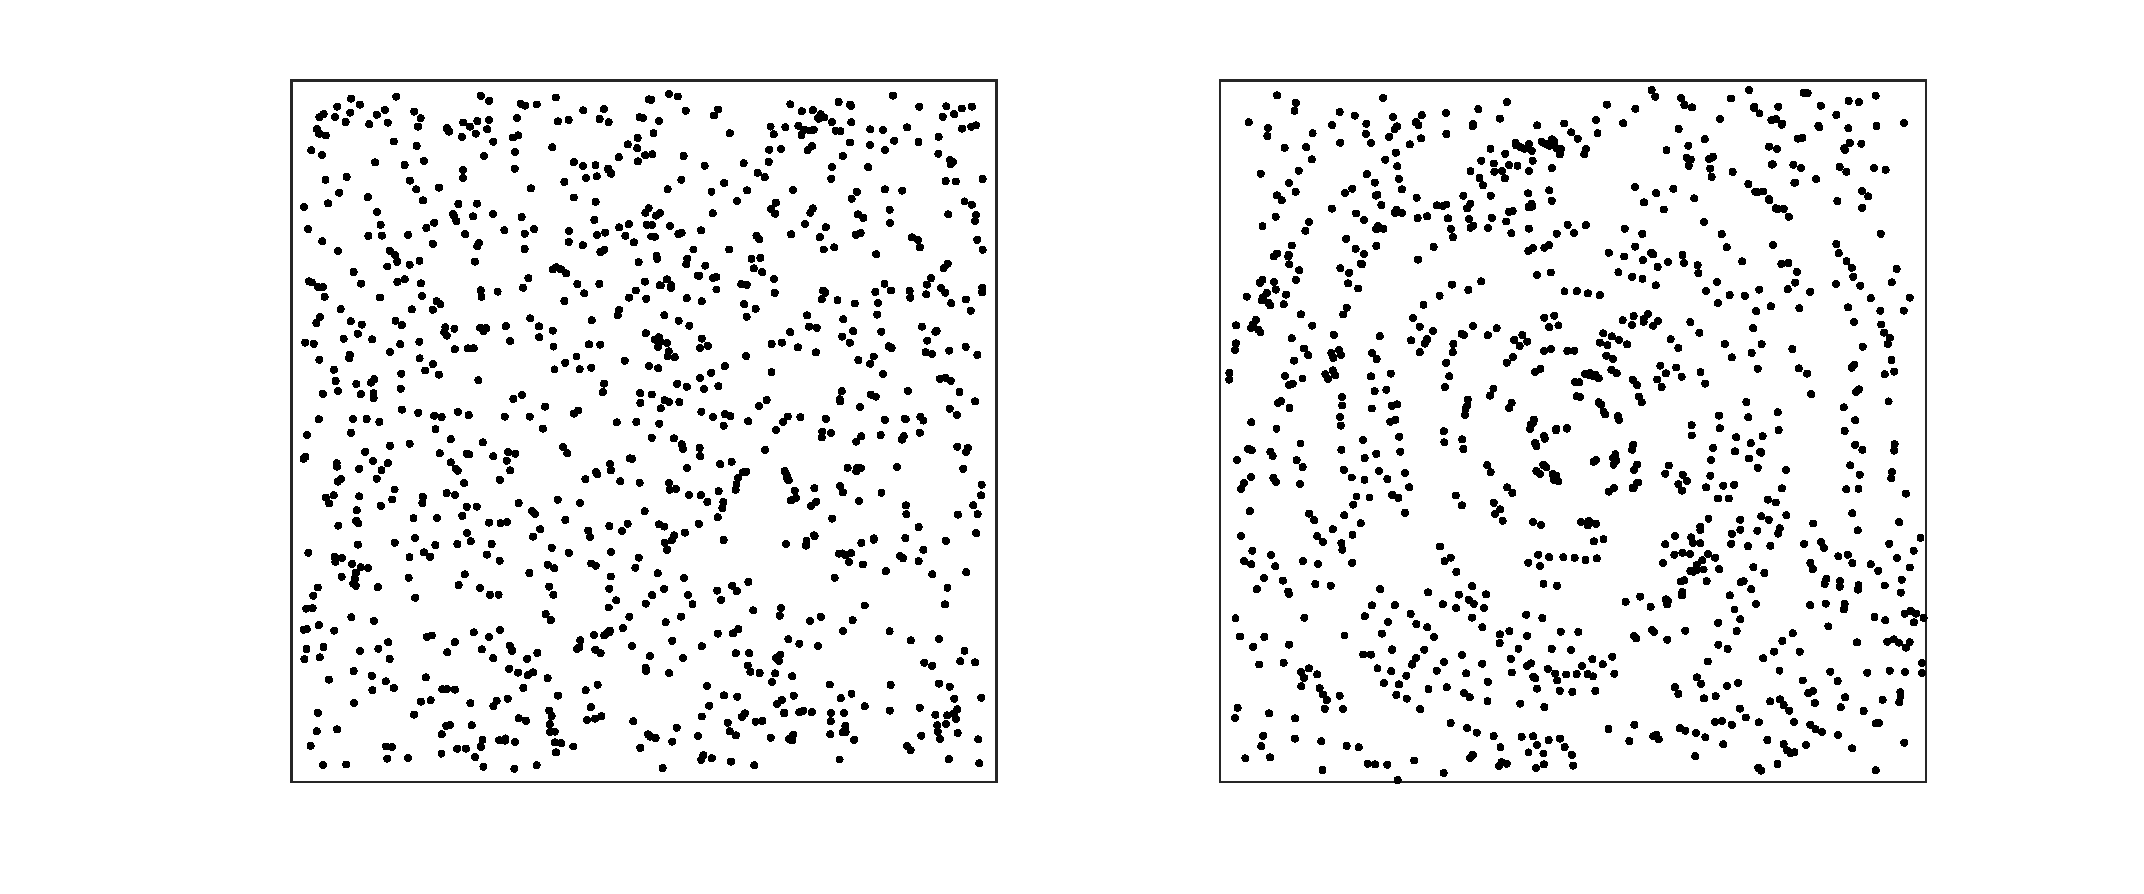
\includegraphics[width=\textwidth]{redundancy}
	\end{center}
\caption[مثالی از رابطه ادراک ساختار با افزونگی]
{
مثالی از رابطه ادراک ساختار با افزونگی -
\textbf{سمت چپ:}
مجموعه‌ای از نقاط نمونه‌برداری شده از یک توزیع یکنواخت دوبعدی.
\textbf{سمت راست:}
نیمی از نقاط از توزیع یکنواخت نمونه‌برداری شده و نیم دیگر با دوران همان نقاط به اندازه پنج درجه حول مرکز توزیع تولید شده است.
\label{fig.redundancy}
}
\end{figure}

به منظور استفاده از این تئوری در
{\mmm{یادگیری بدون نظارت}{unsupervised learning}}،
افزونگی مورد انتظار داده‌های ورودی، کد شده و از خروجی حذف می‌شود.
به این ترتیب، قابلیت اطمینان روش در شناسایی ساختارهای موجود در داده‌های جدید افزایش خواهد یافت.
یادگیری این تبدیل، معادل مدل کردن دانش پیشین در مورد وابستگی‌های آماری موجود در ورودی است%
\cite{barlow_possible_1961}.

در صنایع ارتباطی، کاهش افزونگی یک تکنیک مهم برای کمینه کردن بار ارسالی می‌باشد.
فرستنده پیام، پیش از اینکه پیام را ارسال نماید اطلاعات
{\mmm{افزونه}{redundant}}
موجود در آن را حذف می‌کند تا طول سیگنال کوتاه‌تر شده و با هزینه کمتر قابل ارسال باشد.
اما علاوه بر کاربرد فوق، کاهش افزونگی قابلیت این را دارد که ویژگی‌ها و الگو‌های بامعنی را از داده‌ها استخراج نماید.
به عنوان مثال در مبحث فشرده‌سازی زبان‌های طبیعی، یکی از اقداماتی که می‌توان به منظور ایجاد ویژگی‌های جدیـد انجام داد، ترکیب حروف الفبا و تولید نشانه‌های جدید می‌باشد.
بعضی از این نشانه‌ها احتمال وقوع بیشتری دارند که همان کلمات زبان مورد بررسی هستند.
بنابراین فشرده سازی متن می‌تواند موجب استخراج ویژگی‌های مفهومی مانند کلمات گردد.
در صورتی که این فرایند فشرده‌سازی را بیشتر ادامه دهیم ممکن است دریابیم که احتمال ترکیب بعضی کلمات با بعضی کلمات دیگر در جملات بیشتر است و در نتیجه ساختار جملات را کشف نماییم.

در مورد تصاویر نیز مسئله مشابه است و کاهش افزونگی می‌تواند موجب تشخیص ویژگی‌های جالب توجهی در تصویر گردد.
در این حالت الفبای مورد بررسی، شدت نور پیکسل‌های تصویر بوده و اقدامی که باید انجام شود این است که این پیکسل‌ها را به فضای دیگری تبدیل نماییم به طوری که نتایج از یکدیگر مستقل باشند.
برای مثال فرض شود که یک تصویر از کنار هم گذاشتن بافت‌هایی ساخته می‌شود که از هم مستقل هستند.
فضای پیکسلی تصویری در نتیجه می‌تواند به فضای بافتی تبدیل شود که در آن هر بافت با توجه به محل و اندازه و نوع آن مشخص می‌شود.
نوع بافت می‌تواند با یک مدل آماری مشخص شود.
محل و اندازه بافت با یک متغیر پنهان مشخص می‌شود که  مشخص می‌کند در یک بخش تصویر با چه احتمالی از یک بافت به بافت دیگر تغییر روی می‌دهد.

هدف از این پایان نامه، طراحی مدلی آماری برای تقطیع تصاویر دیجیتال از طریق کاهش افزونگی می‌باشد.
مدل ارائه شده می‌بایست توانایی مدل کردن ویژگی‌های آماری محلی تصاویر را داشته و بتوان با استفاده از استنتاج از متغیر پنهان ارائه شده توسط آن، مرزهای تقطیع تصویر را تعیین نمود.
برای این منظور از
{\mmm{مدل آمیخته}{mixture model}}ای از توزیع‌های
\lr{von Mises-Fisher}
استفاده شده است.
دلیل استفاده از مدل‌های آمیخته، ماهیت توزیع شدت نور پیکسل‌های تصاویر طبیعی در هر یک از بافت‌های موجود در تصویر است.
در تصاویر طبیعی معمولا هر بافت از تعدادی "زیربافت" در مقیاس کوچکتر تشکیل شده است%
~\cite{permuter_study_2006}.
به عنوان مثال می‌توان تصاویر هوایی گرفته شده از یک جنگل با انواع درختان مختلف را در نظر گرفت که بافت هر ناحیه از جنگل از ترکیب بافت‌های مربوط به درختان مختلف تشکیل شده است.
 بنابراین با توجه به این ویژگی، استفاده از مدل‌های آمیخته می‌تواند یک انتخاب مناسب برای مدل کردن بافت‌ها در تصاویر طبیعی باشد.
%TODO maybe use "Some Statistical Properties of Natural Images" from Dr thesis

یکی از دشواری‌های استفاده از مدل‌های آماری در کار با تصاویر طبیعی، مشکل ابعاد بالای پارامترهای مدل است که مشکلات زیادی را هنگام تخمین آن‌ها ایجاد می‌کند.
حتی برای پنجره‌های نسبتا کوچک انتخاب شده از این تصاویر نیز ابعاد پارامترهای مدل لازم برای بازنمایی داده‌ها می‌تواند به شدت بالا رفته و در تخمین چگالی مدل چالش ایجاد کند.
مدل
\lr{von Mises-Fisher}
با توجه به پایین بودن ابعاد پارامترهای آن، می‌تواند انتخاب خوبی برای اجزای مدل آمیخته باشد.


 در ادامه و در فصل
\ref{ch:mixtureModels}
نگاهی به مدل‌های آمیخته و مسائل و مشکلاتی که در عمل برای کار کردن با آن‌ها باید در نظر گرفته شوند خواهیم داشت.
سپس در فصل
\ref{ch:imageSegmentation}
به مرور مسئله تقطیع تصاویر و کارهای انجام شده در این حوزه می‌پردازیم.
همگام با پیشبرد این پروژه، یک بسته نرم‌افزاری جهت کار با مدل‌های آمیخته تهیه شده است که فصل
\ref{ch:mixest}
به معرفی آن اختصاص یافته است.
در فصل
\ref{ch:vMF}
با توزیع
\lr{von Mises-Fisher}
و مدل آمیخته متشکل از این نوع توزیع آشنا شده و الگوریتم پیشنهادی خود برای مقداردهی اولیه به پارامترهای این مدل را شرح خواهیم داد.
فصل
\ref{ch:proposedMethod}
به معرفی روش پیشنهاد شده برای تقطیع تصاویر پرداخته و در فصل
\ref{ch:results}
نتایج آزمایشات و مقایسه آن‌ها با برخی از الگوریتم های مطرح تقطیع تصاویر ارائه می‌شوند.
در انتها و در فصل
\ref{ch:conclusion}
به جمع‌بندی مطالب و بحث در مورد راه‌های ممکن برای بهبود نتایج می‌پردازیم.








\chapter{مدل‌های آمیخته} \label{ch:mixtureModels}
%TODO ref McLachlan book
مدل‌های آمیخته
{\mmm{محدود}{finite mixture models}}
که پس از این به اختصار با عنوان مدل‌های آمیخته به آن‌ها اشاره می‌کنیم، یکی از ابزارهای قدرتمند در آمار و احتمالات جهت مدلسازی گونه‌های مختلفی از پدیده‌های تصادفی هستند.
این مدل‌ها در سال‌های اخیر، به علت  برخورداری از قابلیت انعطاف بالا جهت توصیف توزیع‌های احتمالی پیچیده، توجه پژوهشگران زیادی را در حوزه های مختلف کاربردی و تئوری به خود جلب نموده‌اند.
مدل‌های آمیخته در این کاربردها علاوه بر استفاده مستقیم جهت ارائه مدل توصیفی برای توزیع‌ها، به عنوان مبنا در تکنیک‌های مختلفی مانند
{\mmm{تحلیل خوشه‌ها و طبقه‌بندی پنهان}{cluster and latent class analysis}}،
{\mmm{تحلیل افتراقی}{discriminant analysis}}،
{\mmm{تحلیل تصاویر}{image analysis}} و
{\mmm{تحلیل بقا}{survival analysis}} مورد استفاده قرار می‌گیرند{\cite{mclachlan_finite_2004}}.

با توجه به این که هر توزیع پیوسته‌ای را می‌توان با دقت دلخواه با یک مدل آمیخته محدود از توزیع‌های نرمال با واریانس یا کوواریانس یکسان تخمین زد، مدل‌های آمیخته یک چارچوب
{\mmm{نیمه‌پارامتری}{semiparametric}} مناسب برای مدل کردن شکل‌های ناشناخته توزیع فراهم می‌کنند. مدل‌های آمیخته قابلیت مدل نمودن توزیع‌های کاملا پیچیده را توسط انتخاب مناسب
{\mmm{اجزا}{components}}ی خود جهت بازنمایی دقیق  نواحی محلی
{\mmm{تکیه‌گاه}{support}} توزیع حقیقی دارا هستند.
بنابراین این مدل‌ها می‌توانند در حالاتی که یک خانواده پارامتری واحد قادر به فراهم نمودن یک مدل رضایت‌بخش برای تغییرات محلی در داده‌های مشاهده شده نیست، مفید واقع شوند.

\section{تعاریف اولیه}
تابع چگالی احتمال برای مدل آمیخته به صورت یک جمع وزن داده شده از خانواده‌ای از چگالی‌های پارامتری تعریف می‌شود. به عنوان مثال اگر چگالی احتمال
$f(x|\theta)$
را به عنوان چگالی احتمال اجزای مدل آمیخته در نظر بگیریم که در آن
$\theta$
پارامترهای توزیع را نمایش می‌دهد، چگالی احتمال مدل آمیخته با رابطه زیر مشخص می‌شود:
$$p_X(x)=\sum_{k=1}^{K}w_k f(x|\theta_k).$$

ضرایب
$w_k$
با عنوان
{\mmm{وزن‌های تلفیق}{mixing weights}}
اجزا شناخته می‌شوند.
برای این که
$p_X(x)$
یک تابع چگالی با تعریف درست باشد، وزن‌ها باید مثبت بوده و حاصل جمعشان یک شود:
$$w_k \geq 0,$$
$$\sum_{k=1}^{K}w_k=1.$$

نمونه‌ای از مدل‌های آمیخته که در کاربردهای بسیاری استفاده می‌شود،
{\mmm{مدل آمیخته گوسی}{Gaussian mixture model}}
است که در آن، تابع چگالی $f$ دارای توزیع گوسی با بردار میانگین
$\bm{\mu}$
و ماتریس کوواریانس
$\bm{\Sigma}$
است:
$$p_X(\bm{x})=\sum_{k=1}^{K}w_k (2\pi)^{-\frac{n}{2}}|\bm{\Sigma}|^{-\frac{1}{2}}
 \exp\left(-\frac{1}{2}(\bm{x}-\bm{\mu})^T\bm{\Sigma}^{-1}(\bm{x}-\bm{\mu}) \right).$$

یکی از ویژگی‌های قابل توجه در مدل‌های آمیخته، سادگی تولید نمونه‌های تصادفی از مدل است. برای این منظور کافیست که با احتمال
$w_k$
از جزء $k$ام،
$f(x|\theta_k)$،
نمونه تصادفی تولید شود. مشاهده می‌شود که می‌توان وزن‌های
$w_k$
را به مثابه یک
{\mmm{توزیع پیشین}{prior distribution}}
روی برچسب پنهان جزء مربوطه در نظر گرفت:
$$p_X(x)=\sum_{k=1}^{K}p_K(k)p_X(x|k).$$

\section{مدل آماری استنتاج با توزیع‌های آمیخته}
به منظور انجام استنتاج آماری با استفاده از مدل‌های آمیخته، مسائلی وجود دارد که باید در نظر گرفته شوند.
%TODO figure
اولین نکته‌ای که باید در مدل آماری در نظر گرفته شود این است که مدل باید اطلاعات پیشین ما در مورد داده‌ها را انعکاس دهد که این کار در مدل‌های آمیخته با انتخاب مناسب توزیع‌های احتمال اجزای مدل انجام می‌شود.

تخمین پارامترهای مدل از طریق کمینه یا بیشینه نمودن یک تابع هدف مشخص انجام می‌شود.
یکی از معیارهایی که معمولا در تابع هدف مورد استفاده قرار می‌گیرد و کار تئوری زیادی در خصوص آن انجام شده است، معیار
{\mmm{دیورژانس KL}{KL-divergence}}
است که میزان تطبیق توزیع احتمال مدل را با توزیع حقیقی که داده‌ها از آن گرفته شده‌اند می‌سنجد.
این معیار برآمده از یک درک شهودی در حوزه نظریه اطلاعات است و تعداد بیت اضافی لازم برای کدگذاری داده‌ها در مدل فرض شده را در مقایسه با میزان اطلاعات موجود در داده‌های اصلی مورد اندازه‌گیری قرار می‌دهد.
اگر دو متغیر تصادفی
$\bm{P}$
و
$\bm{Q}$
به ترتیب با توزیع‌های
$p_{\bm{X}}$
و
$q_{\bm{X}}$
داشته باشیم، دیورژانس \lr{KL} بین این دو متغیر تصادفی به صورت زیر تعریف می‌شود:
\begin{eqnarray}\label{eq:kl}
\begin{split}
KL(P \parallel Q) & =\int p_{\bm{X}}(x) \log \frac{p_{\bm{X}}(x)}{q_{\bm{X}}(x)} dx\\
& =\int p_{\bm{X}}(x) \log p_{\bm{X}}(x) dx -
\int p_{\bm{X}}(x) \log q_{\bm{X}}(x) dx.
\end{split}
\end{eqnarray}

در این رابطه قرینه انتگرال اول،
$$H_{\bm{P}}(x) = - \int p_{\bm{X}}(x) \log p_{\bm{X}}(x) dx,$$
آنتروپی توزیع
$p_{\bm{X}}$
است و میزان اطلاعات موجود در آن را اندازه‌گیری می‌کند.
انتگرال دوم،
$$E_{\bm{P}}[-\log q_{\bm{X}}(x)] = \int p_{\bm{X}}(x) \log q_{\bm{X}}(x) dx,$$
{\mmm{آنتروپی متقاطع}{cross entropy}}
بین
$\bm{P}$
و
$\bm{Q}$
است و تعداد بیت‌های مورد نیاز برای کدگذاری داده‌ها در توزیع
$q_{\bm{X}}$
را اندازه گیری می‌کند. دیورژانس \lr{KL} همیشه مقداری نامنفی است و فقط در حالتی که دو متغیر تصادفی
$\bm{P}$
و
$\bm{Q}$
با یکدیگر برابر باشند مقدار صفر خواهد داشت\cite{dembo_information_1991}.

اگر در رابطه \ref{eq:kl} متغیر تصادفی
$\bm{P}$
مربوط به توزیع حقیقی و متغیر تصادفی
$\bm{Q}$
مربوط به توزیع مدل باشد، با جایگزین کردن توزیع مشاهده شده داده‌ها بجای توزیع حقیقی، به سادگی مشاهده می‌شود که
{\mmm{برآورد درست‌نمایی بیشینه}{maximum likelihood estimation}}
هنگامی که اندازه داده‌ها به سمت بی‌نهایت میل کند، مقدار کمینه دیورژانس \lr{KL} را بین توزیع مدل و توزیع حقیقی نتیجه خواهد داد.
%http://www.hongliangjie.com/2012/07/12/maximum-likelihood-as-minimize-kl-divergence/

\section{ملاحظات کاربردی}
الگوریتم بهینه‌سازی استفاده شده برای تخمین پارامترهای مدل، باید ویژگی‌هایی را دارا باشد تا بتوان در عمل از آن استفاده نمود.
یکی از مهمترین این ویژگی‌ها این است که الگوریتم باید از نظر محاسباتی کارآمد باشد یعنی با سرعت قابل قبول به مقادیر بهینه همگرا شود.
در این بخش به بررسی تکنیک‌های مورد نیاز جهت نیل به این مقصود می‌پردازیم.

\subsection{تنظیم در بهینه‌سازی} %TODO footnote "regularization"
یکی از مسائلی که در استفاده از چارچوب درست‌نمایی بیشینه برای تخمین پارامترها باید مورد رسیدگی قرار گیرد، مشکل
{\mmm{تباهیدگی}{degeneracy}}
در تابع لگاریتم درست‌نمایی است به این معنی که ممکن است مقدار لگاریتم درست‌نمایی در بعضی نواحی به سمت بی‌نهایت میل کند.
به عنوان مثال در یک مدل آمیخته گوسی تک‌متغیره:









\chapter{تقطیع تصاویر} \label{ch:imageSegmentation}
%from Zhang book
تکنیک‌های
{\mmm{مهندسی تصاویر}{image engineering}}
را می‌توان به سه لایه کلی تقسیم نمود:
{\mmm{پردازش تصاویر}{image processing}}،
{\mmm{تحلیل تصاویر}{image analysis}}
و
{\mmm{ادراک تصاویر}{image understanding}}%
~\cite{zhang_advances_2006}.
تقطیع تصاویر، اولین گام لازم برای تحلیل تصاویر است و انجام درست آن تاثیر بسزایی در دقت تحلیل خواهد داشت. در تحلیل تصاویر، هدف، استخراج اطلاعات مورد نیاز از تصاویر است که در سه مرحله صورت می‌گیرد: تقطیع تصویر،
{\mmm{بازنمایی اشیا}{object representation}}
و
{\mmm{سنجش مشخصات}{feature measurement}}.

%TODO (from Szeliski p237)
\iffalse
کار مشابه تقطیع تصاویر در علم آمار،
{\mmm{آنالیز خوشه‌ها}{cluster analysis}}
است که پژوهش‌های زیادی روی آن انجام شده و صدها الگوریتم برای آن پیشنهاد شده است.
\fi

تقطیع تصاویر معمولا به این صورت تعریف می‌شود: فرایند تقسیم‌بندی تصویر به بخش‌های تشکیل‌دهنده آن و استخراج بخش‌های مورد نظر (اشیاء).
نتایج تقطیع در کلیه مراحل بعدی تحلیل تصویر مانند بازنمایی، توصیف و سنجش مشخصات اشیا، و حتی فرایندهای سطوح بالاتر مانند طبقه‌بندی اشیا و تفسیر صحنه تاثیرگذار خواهد بود.
اولین تکنیک برای تجزیه تصاویر به بخش‌های تشکیل‌دهنده آن‌ها توسط
\lr{Roberts}
معرفی شد%
~\cite{zhang_advances_2006}.
او یک اپراتور برای آشکارسازی لبه‌های میان بخش‌های مختلف تصویر معرفی کرد که با نام خودش شناخته می‌شود\LTRfootnote{Roberts edge detector}.
پس از آن، تکنیک‌ها و الگوریتم‌های زیادی برای تقطیع تصاویر پیشنهاد شده است.
%from zhu_pixels_2015
در روش‌های اولیه، با الهام از ایده‌های موجود برای خوشه‌بندی، تاکید بر
{\mmm{ادغام}{merge}}
و
{\mmm{انشعاب}{split}}
نواحی به صورت محلی بود%
~\cite{ohlander_picture_1978, brice_scene_1970}.
اما در روش‌های جدید معمولا یک معیار سراسری در کل تصویر بهینه‌سازی می‌شود%
~\cite{comaniciu_mean_2002, felzenszwalb_efficient_2004, shi_normalized_2000, chan_active_2001, beare_locally_2006}.
همچنین روش‌های تقطیع
{\mmm{تعاملی}{interactive}}
پیشنهاد شده‌اند که در کاربردهایی مانند تحلیل تصاویر پزشکی یا ویرایش تصاویر که در آن‌ها مکان‌یابی دقیق اشیاء در تصویر مورد نیاز است، با کمک گرفتن از ورودی کاربر عمل تقطیع را انجام می‌دهند%
~\cite{rother_grabcut_2004, nguyen_robust_2012}.
با پیدایش مجموعه دادگان مقیاس بزرگ برای تصاویر، مانند مجموعه
ImageNet~\cite{deng_imagenet_2009}،
و نیز تصاویر روزافزون به اشتراک گذاشته شده در شبکه‌های اجتماعی اینترنتی، الگوریتم‌های
{\mmm{تقطیع مشترک}{cosegmentation}}
که اشیاء تکرار شده را در مجموعه‌ای از تصاویر جدا می‌کنند، در سال‌های اخیر مورد توجه زیادی قرار گرفته‌اند%
~\cite{rother_cosegmentation_2006, kim_multiple_2012, joulin_multiclass_2012}.

در این مدت همچنین مفهوم و دامنه تصاویر نیز گسترش زیادی یافته است.
به عنوان مثال تصاویر دوبعدی به تصاویر سه‌بعدی و تصاویر ثابت به تصاویر متحرک (ویدئو) و تصاویر
{\mmm{طیف خاکستری}{gray level}}
به تصاویر رنگی و
{\mmm{چندطیفی}{multi-band}}
توسعه پیدا کرده‌اند
که این موضوع به نوبه خود به گسترش مفاهیم و تکنیک‌های تقطیع تصاویر منجر شده است.

می‌توان تقطیع را به صورت افراز تصویر به تعدادی ناحیه ناهمپوشان که اجتماع آنها کل تصویر را می‌سازد در نظر گرفت.
\lr{Haralick}
قوانین زیر را برای نواحی حاصل از تقطیع تصاویر پیشنهاد کرده است%
~\cite{haralick_image_1985}:

\begin{enumerate}
	\item
	هر ناحیه باید از نظر ویژگی‌های مشخصی یکنواخت و همگن باشد.
	\item
	نباید در داخل نواحی، حفره‌های زیادی وجود داشته باشد.
	\item
	تفاوت نواحی مجاور از نظر ویژگی‌هایی که برای هر کدام یکنواخت است، باید به طور معناداری زیاد باشد.
	\item
	مرزهای هر ناحیه باید ساده و غیر مجعد بوده و به طور دقیق مشخص شده باشند.
\end{enumerate}

% Three Levels of Research (p19)
کارهای انجام شده در مورد تقطیع تصاویر، عموما طراحی شگردهایی برای کاربردهای خاص بوده و تا کنون نیز نظریه‌ای عمومی در این خصوص ارائه نشده است.
تحقیقات در این خصوص با جهت‌گیری‌ها و مبانی گوناگون  انجام شده و در نتیجه، الگوریتم‌های تقطیع بسیار متنوعی در ادبیات این حوزه پیشنهاد شده است
که نه هیچ یک را می‌توان به طور عمومی روی کلیه تصاویر اعمال کرد و نه می‌توان گفت که الگوریتم‌های متفاوت، همه برای یک کاربرد خاص مناسب هستند.
در ادامه این فصل به مرور برخی از شناخته‌شده‌ترین روش‌های تقطیع خواهیم پرداخت.


\section{مرور برخی از روش‌های رایج تقطیع}
پژوهش‌های زیادی در دهه‌های اخیر در زمینه تقطیع تصاویر طبیعی انجام شده است.
برخی از آن‌ها توانسته‌اند موفقیت و محبوبیت زیادی کسب کرده و در کاربردهای وسیعی مورد استفاده قرار بگیرند.

ویژگی‌های زیر از خصوصیات مهم شاخص NPR به شمار می‌روند. سه ویژگی اول با شاخص PR مشترک هستند اما ویژگی چهارم مختص معیار NPR می‌باشد.

\begin{description}
	\item[عدم امکان تباهیدگی:]
	هنگامی که تقطیع ورودی قابلیت بازنمایی مناسب با مجموعه تقطیع پایه را نداشته باشد، باز هم مقادیر شباهت در محدوده‌ای معقول خواهند بود.
	\item[عدم نیاز به پیش‌فرض‌های خاص در مورد داده‌ها:]
	برای استفاده از این معیار نیازی نیست که تعداد نواحی یا اندازه آن‌ها در دو تقطیع با هم برابر باشند.
	\item[انطباق‌پذیری پویا با جزئیات:]
	این معیار، در ناحیه‌هایی که در تقطیع دستی مبهم بوده‌اند، تفاوت‌های کوچک در سطح پیکسل را در نظر نگرفته و در نواحی دیگر آن‌ها را جریمه می‌کند.
	\item[نمرات قابل مقایسه:]
	نمراتی که با این معیار به دست می‌آیند، امکان مقایسه بامعنا بین تقطیع‌های تصاویر مختلف و نیز تقطیع‌های مختلف یک تصویر واحد را فراهم می‌کنند.
\end{description}

ارزش و کارایی هر معیار تشابه، مبتنی بر مقدار مرجعی است که نسبت به آن سنجیده می‌شود.
برای مسئله‌ی تقطیع تصاویر، می‌توان این مقدار را برابر مقدار مورد انتظار معیار با استفاده از تغییرات و واریانس موجود در مجموعه 







\chapter{بسته نرم‌افزاری تهیه شده برای کار با مدل‌های آمیخته} \label{ch:mixest}
%TODO tell about why using max lik framework
در فصل
\ref{ch:mixtureModels}
به تعدادی از مشکلات موجود هنگام تخمین پارامترهای مدل‌های آمیخته در چارچوب درست‌نمایی بیشینه اشاره نمودیم.
مهم‌ترین این مشکلات، موارد زیر هستند:

\begin{itemize}
\item 
بی‌کران شدن درست‌نمایی: به عنوان مثال هنگامی که یکی از اجزا تعداد کمی از نقاط نزدیک به هم را در بر می‌گیرد درست‌نمایی به سمت بی‌نهایت میل می‌کند%
~\cite{ciuperca_penalized_2003}.

\item
بیشینه‌های محلی: با توجه به این که تابع لگاریتم درست‌نمایی استفاده شده در تخمین پارامترهای مدل‌های آمیخته به طور معمول دارای نقاط کمینه و بیشینه محلی زیادی است، یافتن نقطه بهینه پیچیده خواهد بود%
~\cite{ueda_split_2000}.

\item
تعداد درست اجزای مدل: در بسیاری از کاربردها می‌بایست تعداد مناسب اجزای مدل آمیخته نیز در کنار پارامترهای آنها تخمین زده شود و این تعداد از قبل مشخص نیست%
~\cite{khalili_variable_2007}.
\end{itemize}

متاسفانه کتابخانه‌های نرم‌افزاری موجود برای کار با مدل‌های آمیخته، امکان رسیدگی به این مشکلات را هنگام استفاده از مدل‌های مخلوط در چارچوب درست‌نمایی بیشینه برای حل مسائل مختلف و به خصوص مسائل با ابعاد بالا و دادگان بزرگ، فراهم نمی‌کنند و پیاده‌سازی راه‌حل‌های مناسب جهت رسیدگی به این مسائل، می‌تواند وقت و انرژی زیادی را از پژوهشگران بگیرد.
لذا با توجه به گستردگی کاربردهای مدل‌های آمیخته در علوم مختلف، بر آن شدیم تا یک کتابخانه نرم‌افزاری منسجم جهت کار با مدل‌های آمیخته به صورت یک
{\mmm{جعبه ابزار}{toolbox}}
در محیط نرم‌افزار \lr{MATLAB} تهیه نماییم که علاوه بر استفاده در پروژه حاضر، امکان استفاده از آن برای عموم پژوهشگران میسر باشد.
جعبه ابزار تهیه شده با عنوان
\lr{MixEst}
و به صورت
{\mmm{متن باز}{open source}}
از طریق آدرس اینترنتی
\lr{\textit{visionlab.ut.ac.ir/mixest}}
در دسترس عموم قرار دارد%
~\cite{hosseini_mixest_toappear}.

\section{معرفی}
جعبه ابزار
MixEst
یک بسته نرم‌افزاری قدرتمند و با کاربری آسان است که بسیاری از راهکارهای جدید ارائه شده جهت رسیدگی به مسائلی که درمورد مدل‌های آمیخته مطرح گردید در آن پیاده‌سازی شده است.
کاربران می‌توانند از این جعبه ابزار به عنوان یک میز آزمایش برای مدل‌های آمیخته استفاده کنند که یک
{\mmm{واسط برنامه‌نویسی نرم‌افزار}{Application Programming Interface (API)}}
ساده و منسجم همراه با انتخاب‌های فراوان جهت انجام انواع پژوهش‌ها با استفاده از این مدل‌ها را برایشان فراهم می‌کند.
در عین حال در پیاده‌سازی الگوریتم‌ها و محاسبات، داشتن کارآیی بالا خصوصا هنگام کار با دادگان بزرگ مورد توجه قرار گرفته و کاربران می‌توانند از این بسته در کاربردهای عملی نیز استفاده نمایند.
فراخوانی این توابع به سادگی به شکل زیر انجام می‌شود:
\begin{latin}
\begin{lstlisting}
data = D.sample(theta, 1000);
\end{lstlisting}
\end{latin}
توضیحات کامل مربوط به توابع مختلف ارائه شده توسط توزیع‌ها در مستندات مربوط به توابع در بسته نرم‌افزاری آمده است.
در این‌جا به طور مختصر، اصول ابتدایی کار با این توابع را بیان می‌نماییم.
دستور بالا، تابع
\mcode{sample}
را از توزیع
\mcode{D}
فراخوانی می‌کند تا تعداد 1000 نمونه تصادفی را از آن توزیع استخراج نماید.
آرگومان
\mcode{theta}
پارامترهای مورد نظر برای توزیع را در بر دارد.
این آرگومان، یک ساختار ساده است که هر فیلد آن متناظر با یکی از پارامترهای توزیع می‌باشد.
به عنوان مثال اگر توزیع مربوطه همان توزیع گوسی دومتغیره که در بالا ساخته شد باشد، می‌توانیم
\mcode{theta}
را به صورت زیر بسازیم:
\begin{latin}
	\begin{lstlisting}
theta.mu = [1; 2];
theta.sigma = [2 1; 3 4];
	\end{lstlisting}
\end{latin}
به این ترتیب یک ساختار پارامتر برای توزیع گوسی دومتغیره با میانگین
(\mcode{mu})
و ماتریس کوواریانس
(\mcode{sigma})
داده شده خواهیم داشت.
همچنین می‌توان ساختارهای پارامتر را از خروجی برخی از توابع ارائه شده توسط توزیع بدست آورد.
به عنوان مثال با فراخوانی تابع
\mcode{randparam}
می‌توانیم یک ساختار پارامتر با مقادیر تصادفی برای کلیه پارامترهای توزیع بسازیم:
\begin{latin}
	\begin{lstlisting}
theta = D.randparam();
	\end{lstlisting}
\end{latin}
همچنین توابع برازش توزیع بر داده‌های مشاهده شده نیز پارامترهای تخمین زده شده را در قالب همین ساختارها بازمی‌گردانند.
نام پارامترهای استفاده شده برای هر توزیع، در مستندات تابع سازنده آن آمده است.

امکانات معمول ارائه شده از طریق ساختارهای توزیع، شامل توابعی برای محاسبه لگاریتم درست‌نمایی و گرادیان آن نسبت به پارامترها یا داده‌ها، توابع مخصوص توزیع به منظور تنظیم بهینه‌سازی و جلوگیری از بیش‌برازش، توابعی برای محاسبه تابع چگالی احتمال، تابع توزیع تجمعی، آنتروپی، توابع معیار اطلاعاتی و ... هستند که در مستندات بسته، توضیحات کاملی در مورد آن‌ها آمده است.

جعبه ابزار
MixEst
شامل پیاده‌سازی تعدادی از توزیع‌های پرکاربرد می‌باشد که در جدول
\ref{table:distributions}
فهرستی از آن‌ها را آورده‌ایم.
\begin{table}[ht]
\caption{توزیع‌های احتمال پیاده‌سازی شده در جعبه ابزار}
\label{table:distributions}
\begin{center}
\begin{small}
\begin{tabular}{cc}
\hline
\textbf{توزیع}
&
\textbf{تابع سازنده}
 \\ \hline
توزیع گوسی (نرمال چندمتغیره) &
\lr{mvnfactory} \\
توزیع آمیخته &
\lr{mixturefactory} \\
توزیع گاما &
\lr{gammafactory} \\
توزیع ECD
\lr{(Elliptically-Contoured Distribution)}
&
\lr{ecdfactory} \\
توزیع vMF
\lr{(von Mises-Fisher)}
&
\lr{vmffactory} \\
توزیع
\lr{Angular Gaussian}
&
\lr{agfactory} \\
توزیع
\lr{Multinomial Logistic} \lr{(MaxEnt Classifier)}
&
\lr{mnlfactory} \\
توزیع فاکتوریل
\lr{(Factorial)}
&
\lr{factorialfactory} \\
توزیع گوسی با تغییر پارامتر
(\cite{hosseini_manifold_2015})
&
\lr{mvn2factory} \\
توزیع آمیخته شرطی
\lr{(Mixture of Experts)}
&
\lr{moefactory} \\
توزیع گوسی شرطی
&
\lr{cmvnfactory} \\
توزیع گوسی شرطی با تغییر پارامتر
(\cite{hosseini_manifold_2015})
&
\lr{cmvn2factory} \\
گیت softmax
&
\lr{softmaxfactory} \\
\hline
\end{tabular}
\end{small}
\end{center}
\end{table}

%%%%%%%%%%%%%%%%%%%%%%%%%%%%%%%
\section{توابع تخمین پارامترها}
\label{sec:estimation_functions}
%%%%%%%%%%%%%%%%%%%%%%%%%%%%%%%
توابع تخمین در جعبه ابزار
MixEst
الگوریتم‌هایی را پیاده‌سازی می‌کنند که پارامترهای بهینه توزیع‌ها را جهت برازش به داده‌های مشاهده شده می‌یابند.
در این بخش به طور مختصر به نحوه کار با این توابع اشاره می‌کنیم.
اطلاعات دقیق‌تر در مورد هر یک از توابع در مستندات جعبه ابزار موجود است.

تابع اصلی برای برازش توزیع‌ها به داده‌ها تابع
\mcode{estimate}
است که در حالت ساده به صورت زیر قابل فراخوانی می‌باشد:
\begin{latin}
	\begin{lstlisting}
theta = D.estimate(data, options);
	\end{lstlisting}
\end{latin}
آرگومان اول ورودی این تابع،
(\mcode{data})\begin{figure}[b!]
	\begin{center}
		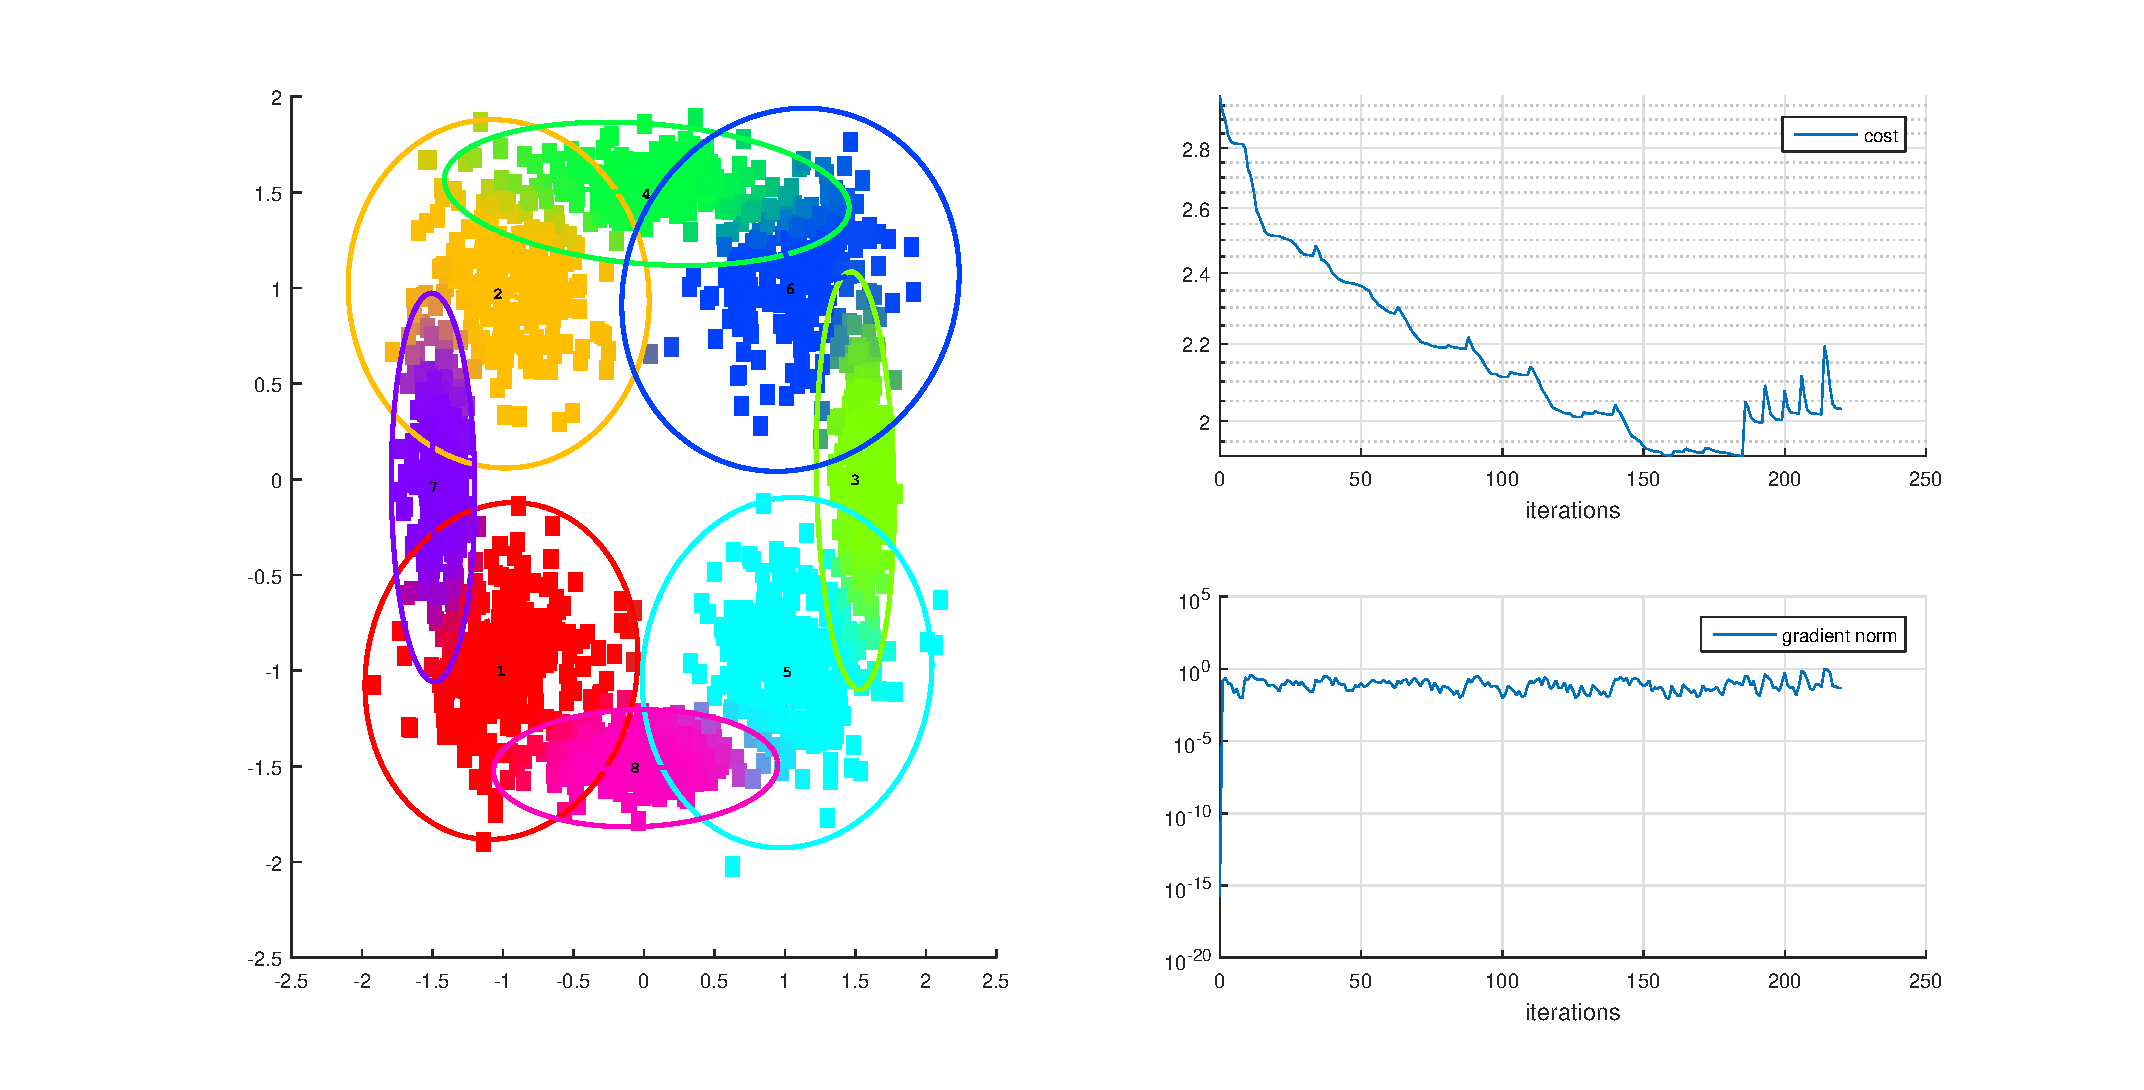
\includegraphics[width=\textwidth]{code-sample2.eps}
	\end{center}
	\caption[نمودارهای خروجی نمونه کد دوم]
	{
نمودارهای خروجی نمونه کد دوم -
نمودار سمت چپ نمایشی بصری از اجزای برازش شده مدل آمیخته گوسی را نشان می‌دهد.
در نمودارهای سمت راست، مقدار تابع هزینه و اندازه گرادیان آن در طی فرآیند تخمین رسم شده است.
		\label{fig.code-sample2}
	}
\end{figure}


\begin{latin}
\begin{lstlisting}[frame=single,numbers=left,aboveskip={\baselineskip},belowskip={1.5\baselineskip}]
load data_sm
% visualization and plotting options
figure('Units', 'normalized', 'OuterPosition', [0 0 1 1])
options.visualization.axes = subplot(2,2,[1 3]);
options.plotCost.axes = subplot(2,2,2);
options.plotCost.iterCount = Inf;
options.plotGradNorm.axes = subplot(2,2,4);
options.plotGradNorm.iterCount = Inf;
options.visualization.mixture.colorize = true;
options.visualization.stopOnClose = true;
% common estimation options
options.verbosity = 1;
options.solver = 'lbfgs';
options.tolCostDiff = 1e-3;
% split-and-merge options
options.sm.splitCriterion = 'kl';
options.sm.mergeCriterion = 'kl';
options.sm.splitInit = 'default';
options.sm.mergeInit = 'default';
options.sm.numInit = 1;
options.sm.numMin = 1;
options.sm.numMax = 15;
options.sm.mergeMaxCands = 5;
options.sm.splitMaxCands = 5;
options.sm.maxFail = 2;
options.sm.ComponentD = mvnfactory2(2);
% run
cem(data, options)
\end{lstlisting}
\end{latin}

\pagebreak %TODO?
در نمونه کد زیر، با استفاده از یک توزیع آمیخته شرطی از توزیع‌های \lr{multinomial logistic}، مجموعه داده \lr{Fisher's Iris} را طبقه بندی می‌نماییم.

\begin{latin}
\begin{lstlisting}[frame=single,numbers=left,aboveskip={\baselineskip},belowskip={1.5\baselineskip}]
% load the iris data and randomly permute them
load data_iris
index = randperm(150);
data = data(:, index);
% Use 120 points for training and 30 for test
data_train = data(:, 1:120);
data_test = data(:, 121:150);
% create a mixture of multivariate logit
datadim = 4; % data dimensions
num = 3; % number of labels
E = mnlfactory(datadim, num); % expert
G = softmaxfactory(num, datadim); % gate
D = moefactory(G, E);
% plotting options
options.plotcost = true;
% main options
options.verbosity = 2;
options.solver = 'lbfgs';
options.tolcostdiff = 1e-6;
options.crossval = true;
options.minibatch.size = 10;
options.maxiter = 200;
options.minibatch.discardhistory = false;
options.crossval.toliter = 100;
% perform estimation
theta = D.estimate(data_train, options);
% perform prediction
data_pred = D.predict(theta, data_test);
label = data_test(end,:)
data_pred
disp(['percentage of correct classification : ' num2str(sum((label-data_pred)==0) * 100 /30)]);
\end{lstlisting}
\end{latin}





\chapter{مدل آمیخته vMF و الگوریتم پیشنهادی برای مقداردهی اولیه آن} \label{ch:vMF}
توزیع
\lr{von Mises Fisher (vMF)}
یکی از توزیع‌های رایج و پرکاربرد برای برازش به
{\mmm{داده‌های جهتی}{directional data}}
%%%%%%%%%%%%%%%%%%%%%%%%%%%%%
\section{الگوریتم k-means++ برای توزیع آمیخته vMF}
%%%%%%%%%%%%%%%%%%%%%%%%%%%%%
\label{sec.kmeanspp}
الگوریتم
\lr{k-means++}
یک روش مقداردهی اولیه احتمالاتی به الگوریتم
\lr{k-means}
می‌افزاید که سعی می‌کند نقاطی از داده‌ها را بیابد که فاصله زیادی از یکدیگر داشته باشند و در عین حال از انتخاب نقاط
{\mmm{برون‌هشته}{outlier}}
اجتناب می‌کند.
در کار با توزیع‌های آمیخته گوسی، نقاط انتخاب شده برای مقداردهی اولیه به میانگین اجزای گوسی مدل استفاده می‌شوند.
برای توزیع‌های آمیخته vMF نیز ما مشابه همین کار را انجام می‌دهیم،
یعنی تعدادی از نقاط داده‌ها را که از یکدیگر دور باشند انتخاب نموده و از آن‌ها برای مقداردهی اولیه به پارامتر
$\vmu$
برای اجزای مختلف مدل استفاده می‌نماییم.

برای این منظور باید یک تابع فاصله مناسب برای نقاط قرار گرفته روی ابرکره واحد تعریف نماییم.
فرض کنید
$\vx$
و
$\vy$
دو نقطه روی ابرکره واحد باشند.
فاصله بین این دو نقطه را به صورت زیر تعریف می‌کنیم:
\begin{equation*}
d(\vx,\vy)= \sqrt{2- 2 \vx^T \vy}.
\end{equation*}
دلیل انتخاب این تابع فاصله در ادامه همین بخش روشن خواهد شد.
الگوریتم
\lr{k-means++}
ابتدا به صورت تصادفی یک نقطه از داده‌ها را به عنوان میانگین اولین خوشه انتخاب می‌کند.
نقطه دوم نیز به صورت تصادفی انتخاب می‌شود، اما با احتمالی متناسب با مربع فاصله از نقطه اول.
به همین ترتیب برای نقطه
$k$ام،
احتمال انتخاب هر نقطه متناسب با کمینه مربع فاصله‌های آن از 
$k-1$
نقطه انتخاب شده قبلی خواهد بود.
جزئیات کامل این روش در الگوریتم~\ref{alg.kmeanspp}
آمده است.

\begin{algorithm}[t]
	\caption{\small \lr{k-means++} برای توزیع آمیخته vMF}
	\label{alg.kmeanspp}
	\begin{algorithmic}
		\begin{latin}
		\STATE \textbf{Input:} $n$ data points on the unit hypersphere $\{\vx_i\}_{i=1}^n$; $K$, the number of components\\
		Set $\vmu_1 \gets \vx_i$, wherein $i\in\{1,...,n\}$ is chosen randomly\\
		Set $c_i \gets \vmu_1^T \vx_i$, $i=1,...,n$ 
		\FOR {$k=2$  to $K$} 
		\item Set $d_i \gets \sum_{j=1}^k (2 - 2 c_j)$, $i=1,...,n$ 
		\item Set $\vmu_k \gets \vx_i$, wherein $i\in\{1,...,n\}$ is chosen by the probability $p_i = d_i/\sum_{i=1}^n{d_i}$
		\item Set  $c_i = \max(c_i, \vmu_k^T \vx_i)$, $i=1,...,n$ 
		\ENDFOR
		\end{latin}
	\end{algorithmic}
\end{algorithm}

در حالت توزیع‌های آمیخته گوسی با تابع فاصله اقلیدسی
$d(\vx,\vy) = \norm{\vx-\vy}$،
در مرجع%
~\cite{arthur_kmeans_2007}
نشان داده شده است که الگوریتم
\lr{k-means++}
یک حد مورد انتظار جالب توجه برای تابع هدف ایجاد می‌کند، در حالی که با مقداردهی اولیه تصادفی، چنین حدی وجود ندارد.
در ادامه نشان خواهیم داد که تابع هدف در خوشه‌بندی قاطع با استفاده از مدل آمیخته vMF 
با پارامترهای تراکم برابر و نیز وزن‌های برابر برای اجزا
(که با نام
{\mmm{توزیع آمیخته vMF کروی}{spherical mixture of vMF distributions}}
شناخته می‌شود%
~\cite{banerjee_clustering_2005})
همان تابع هدف در الگوریتم
\lr{k-means}
است.

برای توزیع‌های آمیخته vMF کروی، تابع هدفی که مورد بیشینه‌سازی قرار می‌گیرد به صورت زیر است:









\chapter{راهکار پیشنهادی برای تقطیع تصاویر}
\label{ch:proposedMethod}
با اتخاذ این فرض که بردارهای ویژگی استخراج شده از تصویر، دارای توزیع آمیخته
\lr{von Mises-Fisher}
هستند، مسئله تقطیع تصویر، به یک مسئله خوشه‌بندی این داده‌ها تبدیل می‌شود.
این خوشه‌بندی بر اساس تئوری اطلاعات و با معیار کاهش
{\mmm{افزونگی}{redundancy}}
به گونه‌ای انجام می‌شود که طول کد لازم برای توصیف کلیه قطعات تصویر، کمینه باشد.
با توجه به اندازه بسیار بزرگ داده‌های مربوط به کل تصویر، ابتدا تصویر را با استفاده از یک الگوریتم تقطیع سطح پایین به تعداد زیادی قطعات کوچک همگن تقسیم می‌کنیم که به آن‌ها
{\mmm{ابرپیکسل}{superpixel}}
می‌گوییم.
سپس با آغاز از این ابرپیکسل‌ها و ادغام پی‌درپی نواحی مجاور با معیار کاهش افزونگی
مبتنی بر درست‌نمایی مدل آمیخته برازش شده بر قطعات، تقطیع نهایی بر اساس بافت‌های تصویر بدست می‌آید.

به منظور بهبود کارایی در راهکار پیشنهادی، از الگوریتم مقداردهی اولیه\section{شبه‌کد}
فرآیند کامل تقطیع با روش پیشنهادی به صورت شبه‌کد در الگوریتم%
~\ref{alg.full_algorithm}
آمده است.

\begin{algorithm}[htb]
	\caption{\small فرآیند کامل تقطیع پیشنهاد شده}
	\label{alg.full_algorithm}
	\begin{algorithmic}
		\begin{latin}
\STATE \textbf{Input:} Image $I$ of height $H$ and width $W$, window size $w$, model component count $K$, model coding-length multiplier $\lambda$.

\STATE Partition $I$ into superpixels $\mathcal{X}_1,\dots,\mathcal{X}_Q$. For pixel $p_i \in \mathcal{X}_j$ initialize its label $l_i=j$.

\STATE Construct a region-adjacency graph $G\{1\},\dots,G\{Q\}$ for the $Q$ segments $\mathcal{X}_1,\dots,\mathcal{X}_Q$.

\STATE Sample $w \times w$ windows for each pixel, and construct feature vectors.

\FORALL {initial segments $\mathcal{X}_i, i=1,\dots,Q$}

\STATE Estimate the parameters, $\theta_i$, of a mixture of $K$ von-Mises Fisher distributions fitting $\mathcal{X}_i$.

\STATE Compute the coding length for the $i$th segment, $L(\theta_i,\mathcal{X}_i)$.

\FORALL {$j \in G\{i\}$}

	\STATE Estimate the parameters, $\theta_{ij}$, of a mixture of $K$ von-Mises Fisher distributions fitting $\mathcal{X}_i \cup \mathcal{X}_j$.
	
	\STATE $U_{ij} \gets L(\theta_i,\mathcal{X}_i) + L(\theta_j,\mathcal{X}_j) - L(\theta_{ij},\mathcal{X}_i \cup \mathcal{X}_j)$.

\ENDFOR

\WHILE {$U_{ij} \gets \max \{U\} > 0$}

	\STATE Merge $\mathcal{X}_i$ and $\mathcal{X}_j$. Update arrays $l$, $G$, $L$ and $U$.
	
	\STATE $Q \gets Q-1$.

\ENDWHILE

\ENDFOR

\STATE \textbf{Output:} Final pixel labels $l_1,\dots,l_{H \times W}$.

		\end{latin}
	\end{algorithmic}
\end{algorithm}










\chapter{نتایج و مقایسه} \label{ch:results}
در این فصل نتایج آزمایش‌های کیفی و کمی انجام‌شده با روش پیشنهاد شده برای تقطیع تصاویر خواهد آمد و نتایج کمی با تعدادی از الگوریتم‌های رایج در این حوزه مورد مقایسه قرار می‌گیرند.

\section{ارزیابی کیفی}
ابتدا به صورت بصری به بررسی نتایج روی مجموعه داده برکلی می‌پردازیم.
شکل
\ref{fig.testlambda}
نتایج تقطیع را با سه مقدار مختلف این پارامتر نمایش می‌دهد.
نتایج تقطیع به صورت "تصویر مصنوعی" نمایش داده شده‌اند.
در این تصاویر، به منظور نمایش بهتر قطعات، هر قطعه با رنگ متوسط پیکسل‌های موجود در آن پر شده است.
مشاهده می‌کنیم که برای مقادیر کوچک پارامتر
$\lambda$
قطعات کمتر با یکدیگر ادغام می‌شوند و بسیاری از ابرپیکسل‌های اولیه بدون تغییر باقی می‌مانند.
اما با افزایش مقدار پارامتر
$\lambda$،
ادغام‌های بیشتری صورت گرفته و اندازه قطعات بزرگ‌تر می‌شود.
با توجه به این که در محاسبه طول کد مربوط به هر قطعه،
$\lambda$
ضریب جمله نمایانگر طول کد مورد نیاز برای بازنمایی پارامترهای مدل است، این امر قابل پیش‌بینی بود،
زیرا این طول کد به ازای هر قطعه، به مجموع طول کد افزوده می‌شود و 
بنابراین ضریب بزرگ برای آن همراه با تعداد قطعات زیاد، طول کد کل را بیشتر از حالتی می‌کند که قطعات بزرگ با درست‌نمایی پایین‌تر داشته باشیم.




\begin{figure}[tp]
	\makebox[\linewidth][c]{%
		\begin{subfigure}[b]{.5\textwidth}
			\centering
			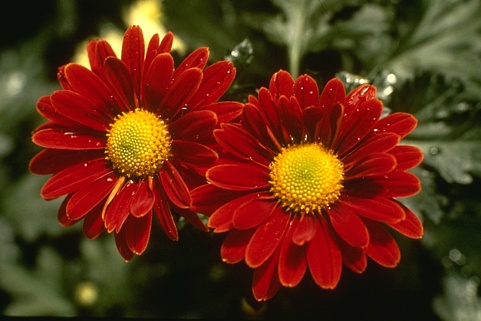
\includegraphics[width=.95\textwidth]{testlambda/original}
			\caption{تصویر اصلی}
		\end{subfigure}%
		\begin{subfigure}[b]{.5\textwidth}
			\centering
			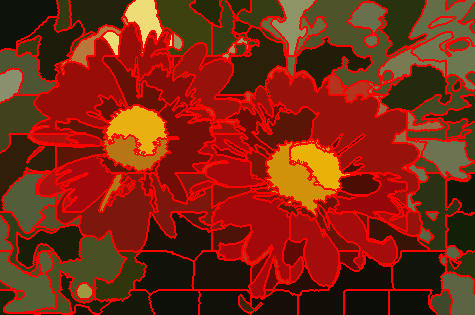
\includegraphics[width=.95\textwidth]{testlambda/10}
			\caption{$\lambda=10$}
		\end{subfigure}%
	}\\[20pt]
	\makebox[\linewidth][c]{%
		\begin{subfigure}[b]{.5\textwidth}
			\centering
			
\includegraphics[width=.95\textwidth]{testlambda/100}
			\caption{$\lambda=100$}
		\end{subfigure}%
		\begin{subfigure}[b]{.5\textwidth}
			\centering
			
\includegraphics[width=.95\textwidth]{testlambda/1000}
			\caption{$\lambda=1000$}
		\end{subfigure}%
	}
	\caption{
مقایسه تاثیر مقادیر مختلف پارامتر
$\lambda$
بر کیفیت تقطیع
		\label{fig.testlambda}
	}
\end{figure}





به منظور بررسی بهتر مراحل اجرای الگوریتم،
نتایج اجرای الگوریتم روی دو نمونه از تصاویر مجموعه برکلی در شکل
\ref{fig.sampleOutputs}
آمده است.
شکل‌های ردیف بالا تصاویر اصلی و
شکل‌های ردیف دوم، ابرپیکسل‌های استخراج شده از آن‌ها را نمایش می‌دهند.
پارامترهای الگوریتم SLIC را به گونه‌ای تنظیم نموده‌ایم که به طور تقریبی تعداد 100 ابرپیکسل استخراج شود.
شکل‌های ردیف سوم، نتایج نهایی اجرای الگوریتم پیشنهادی را نمایش می‌دهند و در ردیف آخر، به منظور نمایش بهتر قطعات، تصاویر مصنوعی ساخته شده توسط آن‌ها آمده است.
برای کسب این نتایج، پارامتر
$\lambda$
برابر 100 در نظر گرفته شده است.
استخراج بردارهای ویژگی با پنجره‌های
7$\times$7
انجام شده و مولفه‌ی DC بردارها حذف گردیده است.
مدل آمیخته برازش شده به داده‌های هر قطعه از تصویر، دارای پنج جزء با توزیع vMF بوده و پارامترهای آن پس از مقداردهی اولیه با الگوریتم
\lr{k-means++}،
با روش EM تخمین زده شده است.


\begin{figure}[!tp]
	\makebox[\linewidth][c]{%
		\begin{subfigure}[b]{.5\textwidth}
			\centering
			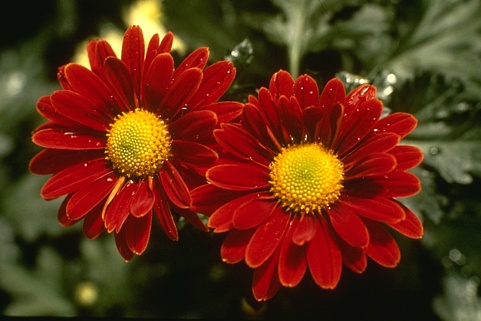
\includegraphics[width=.95\textwidth]{first/124084}
			%\caption{}
		\end{subfigure}%
		\begin{subfigure}[b]{.5\textwidth}
			\centering
			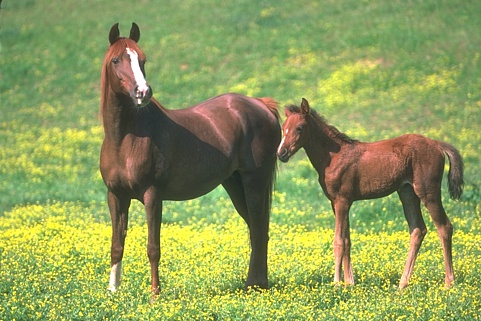
\includegraphics[width=.95\textwidth]{first/113016}
			%\caption{}
		\end{subfigure}%
	}\\
	\makebox[\linewidth][c]{%
		\begin{subfigure}[b]{.5\textwidth}
			\centering
			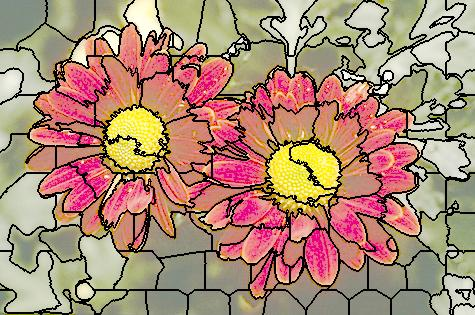
\includegraphics[width=.95\textwidth]{first/124084-sp}
			%\caption{}
		\end{subfigure}%
		\begin{subfigure}[b]{.5\textwidth}
			\centering
			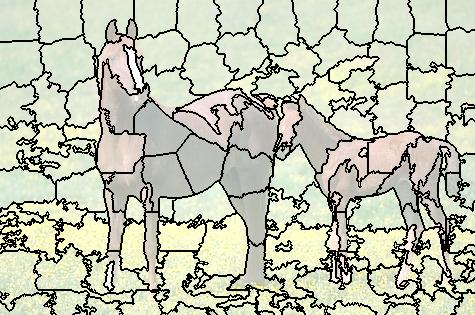
\includegraphics[width=.95\textwidth]{first/113016-sp}
			%\caption{}
		\end{subfigure}%
	}\\
	\makebox[\linewidth][c]{%
		\begin{subfigure}[b]{.5\textwidth}
			\centering
			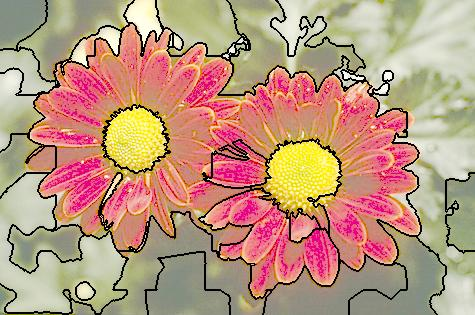
\includegraphics[width=.95\textwidth]{first/124084-result}
%			\caption{}
		\end{subfigure}%
		\begin{subfigure}[b]{.5\textwidth}
			\centering
			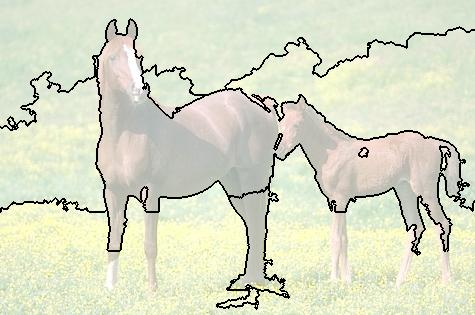
\includegraphics[width=.95\textwidth]{first/113016-result}
%			\caption{}
		\end{subfigure}%
	}\\
	\makebox[\linewidth][c]{%
		\begin{subfigure}[b]{.5\textwidth}
			\centering
			
\includegraphics[width=.95\textwidth]{first/124084-synthetic}
			%\caption{}
		\end{subfigure}%
		\begin{subfigure}[b]{.5\textwidth}
			\centering
			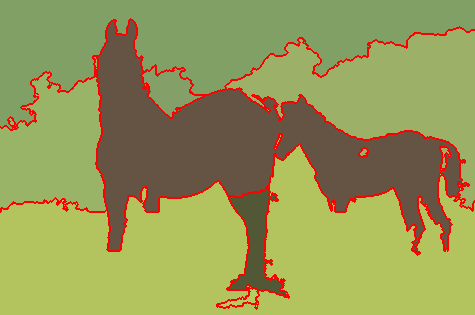
\includegraphics[width=.95\textwidth]{first/113016-synthetic}
			%\caption{}
		\end{subfigure}%
	}
\caption[
نمونه نتایج الگوریتم پیشنهادی روی دو تصویر نمونه
]{
نمونه نتایج الگوریتم پیشنهادی روی دو تصویر نمونه - به ازای هر تصویر (ردیف بالا)، ابرپیکسل‌های استخراج شده با تعداد تقریبی 100 ابرپیکسل (ردیف دوم) و نتیجه نهایی پس از ادغام ابرپیکسل‌ها با پارامتر
$\lambda=100$
(ردیف سوم و چهارم) آمده است.
در ردیف چهارم برای نمایش بهتر، تصاویر مصنوعی حاصل از پر کردن هر قطعه با رنگ متوسط پیکسل‌های موجود در آن آمده است.
\label{fig.sampleOutputs}
}
\end{figure}






محاسبه شده است.

\begin{table}[bh]
	\caption[بررسی مقادیر بهبود طول کد در ادغام قطعات]
	{
بررسی مقادیر بهبود طول کد در ادغام قطعات.
مقادیر بر حسب میلیون واحد اطلاعاتی مبتنی بر لگاریتم طبیعی
(\lr{nat})
هستند.
	}
	\phantomsection
	\label{table.improvement_comparison}
	\begin{center}
		{\setlength{\extrarowheight}{5pt}%
			\begin{tabular}{rcccccc}
				\hline%\cline{1-4}
				&
				\multicolumn{2}{c}{$\lambda=10$}
				&
				\multicolumn{2}{c}{$\lambda=100$}
				&
				\multicolumn{2}{c}{$\lambda=1000$}
				\\
				\textbf{تصویر \hspace{30pt}}
				&
				\textbf{هم‌اندازه}
				&
				\textbf{غیرهم‌اندازه}
				&
				\textbf{هم‌اندازه}
				&
				\textbf{غیرهم‌اندازه}
				&
				\textbf{هم‌اندازه}
				&
				\textbf{غیرهم‌اندازه}
				\\[5pt]\hline
مرمر
& 0.1257    & 0.1696    & 0.2074    & 0.2448    & 1.0242    & 0.9963\\
آلی
& 0.0061-    & 0.0352    & 0.0766    & 0.1101    & 0.9028    & 0.8592\\
سنگ
& 0.1688-    & 0.0465   & 0.0844-    & 0.1213    & 0.7602    & 0.8692\\
چوب
& 0.0356    & 0.0763    & 0.1175    & 0.1521    & 0.9363    & 0.9099
				\\\hline
			\end{tabular}
		}
	\end{center}
\end{table}

همان‌طور که طبق مشاهدات قبلی نیز انتظار می‌رفت، مقادیر بهبود طول کد حاصل از ادغام، با افزایش مقدار پارامتر
$\lambda$
افزایش می‌یابد.
متاسفانه ارتباط معناداری بین مشابهت ظاهری بافت‌های مورد آزمایش و میزان بهبود طول کد ناشی از ادغام آن‌ها در نتایج مشاهده نمی‌شود،
اما واضح شد که تنظیم دقیق پارامتر
$\lambda$
مورد نیاز برای ادغام یا عدم ادغام قطعات مختلف تصاویر، می‌تواند بستگی زیادی به نوع بافت‌های موجود در نواحی مختلف تصویر داشته باشد و احتمالا یک روش انطباق‌پذیر برای تنظیم این پارامتر مشابه کار انجام شده در مرجع
\cite{yang_unsupervised_2008}
می‌تواند در بهبود نتایج موثر باشد.
اما با توجه به زمان نسبتا بالای اجرای الگوریتم پیشنهادی، فعلا موفق نشدیم این بررسی را انجام دهیم.





\chapter{جمع‌بندی} \label{ch:conclusion}
در این بخش ابتدا به جمع‌بندی کارهای انجام شده می‌پردازیم. سپس، پیشنهادهایی برای تکمیل پروژه ارائه می‌کنیم.

\section{کارهای انجام شده}
در این پژوهش روشی برای تقطیع تصاویر مبتنی بر کاهش افزونگی پیشنهاد شد.
بردارهای ویژگی استخراج شده از بافت‌های تصویر با توزیع آمیخته
\lr{von Mises-Fisher}
مدل شد.
در الگوریتم پیشنهادی، ابتدا تصویر با یک الگوریتم تقطیع سطح پایین به تعداد زیادی ابرپیکسل تقطیع شده و با برازش مدل به بردارهای ویژگی و تعریف طول کد لازم برای بازنمایی قطعات با معیار کاهش افزونگی مبتنی بر درست‌نمایی مدل، قطعات مجاور، با هدف کاهش طول کد کل با یکدیگر ادغام می‌شوند.



یک بسته نرم‌افزاری جهت تسهیل کار با مدل‌های آمیخته در ضمن کار روی پروژه تهیه شد که امکانات بسیاری برای پژوهشگران در برازش این مدل‌ها به داده‌های مورد پژوهش فراهم می‌کند.
ویژگی اختصاصی این جعبه ابزار، امکان استفاده از
بهینه‌سازی ریمانی می‌باشد که قابلیت اجرای الگوریتم‌های مبتنی بر گرادیان و انواع تکنیک‌های مرتبط با آن‌ها را برای کاربر فراهم می‌آورد.
این قابلیت می‌تواند راه را برای استفاده از مدل‌های آمیخته در مسائل با مقیاس بزرگ هموار سازد.

همچنین الگوریتم
\lr{k-means++}~\cite{arthur_kmeans_2007}
برای مقداردهی اولیه پارامترهای توزیع آمیخته vMF در بهینه‌سازی، تعمیم داده شد و حد بالایی برای تابع هزینه بهینه‌سازی مورد اثبات قرار گرفت.



\section{کارهای آینده}
\iffalse
با توجه به تاثیر پارامتر
$\lambda$
بر اندازه قطعات ایجاد شده، احتمالا طراحی یک الگوریتم برای تنظیم انطباق‌پذیر این پارامتر به گونه‌ای که در نواحی دارای جزئیات بالا در تصویر مقدار آن کاهش یافته و در نواحی گسترده و با جزئیات کمتر، مقدار پارامتر افزایش یابد می‌تواند در کیفیت بهتر قطعات ایجاد شده تاثیرگذار باشد.
\fi

در این پژوهش ما فقط مسئله تقطیع بدون نظارت تصاویر طبیعی را مورد مطالعه قرار دادیم.
اما چارچوب پیشنهاد شده قابلیت تعمیم به یادگیری با نظارت را نیز داراست.
به نظر ما نگاه به مسئله تقطیع تصاویر از منظر کاهش افزونگی می‌تواند در بهبود درک ما از تقطیع طبیعی تصاویر توسط موجودات زنده مفید باشد.
این ادراک می‌تواند بینش خوبی برای حل مسائل مهم بینایی ماشین مانند
{\mmm{کشف اشیای برجسته}{salient object detection}}،
{\mmm{مرتب‌سازی ادراکی}{perceptual organization}} و
{\mmm{ادراک و حاشیه‌نویسی تصاویر}{image understanding and annotation}}
برای پژوهشگران این حوزه داشته باشد.

در خصوص بسته نرم‌افزاری تهیه‌شده، فضای فراوانی برای توسعه وجود دارد.
به عنوان مثال می‌توان به پیاده‌سازی انواع توزیع‌ها و الگوریتم‌های تخمین پارامتر،
پشتیبانی از جزئیات کاربردهای گوناگون مدل‌های آمیخته در حوزه‌های مختلف
و نیز گسترش محیط‌های نرم‌افزاری پشتیبانی‌شده توسط این مجموعه اشاره نمود.






\cleardoublepage
\bibliography{Dissertation}

% glossaries
\settextfont[Scale=1]{XB Niloofar}
\setlatintextfont[Scale=1]{Times New Roman}
\baselineskip=.75cm
\twocolumn{}
\RTLdblcol
\printglossary[type=FaToEn,style=mylistFa]
\clearpage
\LTRdblcol % note: this should come after a clearpage
\printglossary[type=EnToFa,style=mylistEn]
\onecolumn{}
\defaultfonts

% english pages
\cleartoleftpage % go to a left-sided page
\thispagestyle{empty}
\begin{latin} % xepersian enviorment

\baselineskip=1.5cm
%\chapter*{\centerline{Abstract}}
\parbox{\linewidth}{\centering \textbf{\Large{Abstract}}}
\noindent
In this research, we cast natural-image segmentation as a problem of clustering feature vectors extracted from image textures.
We model the distribution of the texture features using a mixture of von Mises-Fisher distributions.
In the proposed algorithm, by fitting these models to the data we segment the image using an agglomerative clustering algorithm based on the likelihood of the fit.
We conduct comprehensive experiments to measure the performance of the algorithm in terms of visual evaluation and a variety of quantitative indices, and we also compare it to other well-known image-segmentation methods.
While moving the project forward, we have also developed a software package for working with mixture models, which provides the facilities required to estimate the parameters of these models.

\vspace{1cm}
\noindent
\textbf{Keywords:} \textit{Image segmentation; Texture segmentation; Mixture models; von Mises-Fisher distribution; Clustering; MATLAB toolbox; manifold optimization}

\baselineskip=1cm

\end{latin}

\cleartoleftpage % go to a left-sided page
\thispagestyle{empty}
\ignorespaces
\begin{center}
\begin{latin}
	\begin{table}
		\begin{adjustwidth}{1cm}{2.5cm} % using changepage package to locally change the margins
			\begin{tabular}{ccc}
				%\hline
				
\includegraphics[height=1in]{UT-logo-blue}
				&
				\begin{minipage}{0.55\linewidth}
					\begin{center}
						{\Large
University of Tehran
							\\* [0.5cm]
Faculty of Engineering\\ [0.5cm]
Department of Electrical and Computer Engineering
						}
						\\*[1cm]
					\end{center}
				\end{minipage}
				&
				
\includegraphics[height=1in]{ENG-logo-blue}\\
				%\hline
			\end{tabular}
		\end{adjustwidth}
	\end{table}
	\null
	\vskip 1cm
	\textbf{\LARGE{\titleEn}}
	\vskip 2cm
	\LARGE{By:}
	\\ [0.4cm] \Large{\authorEn}
	\vskip 1.5cm
	\LARGE{Under Supervision of:}
	\\ [0.4cm] \Large{\supervisorEn}
	\vskip 1.5cm
	\LARGE{Consulting Advisor:}
	\\ [0.4cm] \Large{\advisorEn}
	\vskip 2cm
	{\normalsize Thesis submitted to the Graduate Studies Office
	in partial fulfillment of the requirements for
	the degree of
	\degreeEn
	\\
	in
	\majorEn}
	\vskip 1cm
	\large{\dateEn}
\end{latin}
\end{center}
\clearpage


\end{document}
